\documentclass[10pt,pr,twocolumn,showpacs,amssymb,floatfix,superscriptaddress]{revtex4-1}
\usepackage{amsmath,graphics,epsfig,mathrsfs}
\usepackage{bm}
\usepackage{epigraph}
\usepackage[]{color} 
%\usepackage{subcaption}
%%%%%% Definition of new commands for abbrevation%%%%%
\newcommand{\lowsub}[1]
{\ensuremath\raisebox{-.4\height}{#1}}
% Fonts
\newcommand{\mbb}{\mathbb}
\newcommand{\mb}{\mathbb}
\newcommand{\mbf}{\mathbf}
\newcommand{\mac}{\mathcal}
\newcommand{\msc}{\mathscr}
\newcommand{\tx}{\text}
\newcommand{\ti}{\textit}
\newcommand{\tb}{\textbf}
\newcommand{\tsf}{\textsf}
\newcommand{\tm}{{\times}}
\newcommand{\noi}{\noindent}
% Symbols
\newcommand{\dg}{\dagger}
\newcommand{\daw}{\downarrow}
\newcommand{\dna}{\downarrow}
\newcommand{\dn}{\downarrow}
\newcommand{\Dna}{\Downarrow}
\newcommand{\la}{\langle}
\newcommand{\law}{\leftarrow}
\newcommand{\lra}{\leftrightarrow}
\newcommand{\nn}{\nonumber}
\newcommand{\pat}{\partial}
\newcommand{\para}{\parallel}
\newcommand{\pr}{\prime}
\newcommand{\ra}{\rangle}
\newcommand{\raw}{\rightarrow}
\newcommand{\til}{\tilde}
\newcommand{\upa}{\uparrow}
\newcommand{\up}{\uparrow}
\newcommand{\Upa}{\Uparrow}
\newcommand{\ub}{\underbrace}
\newcommand{\fr}{\frac}
%Greek letters
\newcommand{\alp}{\alpha}
\newcommand{\dlt}{\delta}
\newcommand{\Dlt}{\Delta}
\newcommand{\Dt}{\Delta}
\newcommand{\eps}{\epsilon}
\newcommand{\gm}{\gamma}
\newcommand{\Gm}{\Gamma}
\newcommand{\lam}{\lambda}
\newcommand{\Lam}{\Lambda}
\newcommand{\vp}{\varphi}
\newcommand{\tha}{\theta}
\newcommand{\vth}{\vartheta}
\newcommand{\vps}{\varepsilon}
\newcommand{\vs}{\varsigma}
\newcommand{\og}{\omega}
\newcommand{\Og}{\Omega}
\newcommand{\sg}{\sigma}
\newcommand{\Sg}{\Sigma}
\newcommand{\sig}{\sigma}
\newcommand{\kp}{\kappa}
\newcommand{\h}{\hat}
%Others
\newcommand{\etal}{{\em et al.,~}}
\newcommand{\ie}{{i.e.,~}}
%\usepackage{wrapfig}
\include{rgb.tex}
\usepackage{xcolor}
\usepackage[percent]{overpic}
\usepackage{tikz}
\usepackage{hyperref}
\hypersetup{backref=true,pagebackref=true,hyperindex=true,colorlinks=true,citecolor=blue, breaklinks=true,urlcolor=
cyan,linkcolor=blue,bookmarks=true,bookmarksopen=true}

\begin{document}
\title{ Rashba spin-orbit effects in tunnel junctions with magnetic insulators}


\author{Collins Ashu Akosa}
\affiliation{Department of Applied Physics, Waseda University, Okubo, Shinjuku-ku, Tokyo 169-8555, Japan}
\affiliation{RIKEN Center for Emergent Matter Science (CEMS), 2-1 Hirosawa, Wako, Saitama 351-0198, Japan}
\affiliation{Department of Theoretical and Applied Physics, African University of Science and Technology (AUST), Km 10 Airport Road, Galadimawa, Abuja F.C.T, Nigeria}
%
\author{Christian Ortiz Pauyac}
\affiliation{RIKEN Center for Emergent Matter Science (CEMS), 2-1 Hirosawa, Wako, Saitama 351-0198, Japan}
%
%
%\author{Sergey Nikolaev}
%\affiliation{WRHI, Tokyo Institute of Technology, Yokohama 226-8503, Japan}
%
\author{Mairbek Chshiev}
\affiliation{Univ. Grenoble Alpes, CNRS, CEA, SPINTEC, Grenoble 38000, France}
\affiliation{Institut Universitaire de France (IUF), Paris, 75231, France}

%\author{Alan Kalitsov}
%\affiliation{Western Digital, San Jose, California 95131, USA}
%
\author{Gen Tatara}
\affiliation{RIKEN Center for Emergent Matter Science (CEMS), 2-1 Hirosawa, Wako, Saitama 351-0198, Japan}

\author{Masahito Mochizuki}
\affiliation{Department of Applied Physics, Waseda University, Okubo, Shinjuku-ku, Tokyo 169-8555, Japan}

\date{\today}




\begin{abstract}
In the framework of Keldysh formalism and the tight-binding model, we investigate spin-orbit phenomena such as the anomalous and spin Hall effects, tunneling anisotropic magnetoresistance, 
and Rashba-induced torque in two categories of tunnel junctions: 
i) normal metal/non-magnetic insulator/ferromagnetic metal and ii) normal metal/ferromagnetic insulator/normal metal. 
Our findings reveal a notable enhancement, approximately by one order of magnitude, of the tunneling anisotropic
magnetoresistance and the angular dependence of the spin Hall effect when considering a ferromagnetic insulator instead of a ferromagnetic metal. Moreover, the former effect exhibits greater magnitude in asymmetric junctions.
The Rashba torque and the anomalous Hall effect, in contrast, are comparable in magnitude for both types of systems. 
In the presence of a ferromagnetic lead these effects change sign as the system moves from the half metallic to the low band filling regime, whereas in the presence of a ferromagnetic insulator no sign reversal is present as a result of the spin filtering process in the ferromagnetic barrier. The validity of the model is supported with first principles calculations.
\end{abstract}
\pacs{10.1103.Jk}
\maketitle


The exploration of spin-orbit coupling (SOC), which correlates the momentum of the electron with its spin, 
has given rise to a new field known as spin-orbitronics. This field focuses on the manipulation of non-equilibrium material properties via SOC \cite{rashba,Soumyanarayanan2016,Manchon2019}. Spin-orbitronics has garnered particular attention in metallic and semiconducting systems due to its role in the reciprocal conversion of spin and charge currents. 
 Spin-orbit coupling arises from both extrinsic and intrinsic sources. Extrinsic contributions stem from spin-orbit-coupled impurities in the system, while intrinsic 
 effects result from spin-orbit interactions in the material's band structure. In low-dimensional multilayered structures, the intrinsic effect, referred to as Rashba SOC, emerges from the breaking of structural inversion symmetry. The Rashba SOC has been extensively studied in systems with a current-in-plane configuration, including III-V semiconductor materials \cite{sc}, bilayer junctions comprising heavy metals and ferromagnetic metals \cite{miron}, graphene layers on metallic substrates \cite{slg}, 2D topological insulators \cite{ti}, and 2D van der Waals heterostructures \cite{tmd}.




In this work, we investigate a distinct configuration where the current flows perpendicular to the plane focusing on two types of single-barrier tunnel junctions. The first one comprises a ferromagnetic insulating barrier (FI) sandwiched between normal metal leads (NM), denoted as NM/FI/NM. In the other case, the barrier is non-magnetic (I), and the right lead is a ferromagnetic metal (FM), represented as NM/I/FM. In both configurations, the right interface is subjected to an interfacial Rashba SOC. Previous studies have demonstrated that in conventional and semi-magnetic tunnel junctions, specifically FM/I/FM and NM/I/FM configurations, respectively, Rashba SOC gives rise to interesting phenomena such as the anomalous and spin Hall effects (AHE and SHE) \cite{ahe-she}, anisotropic tunneling magnetoresistance (ATMR) \cite{atmr0}, tunneling anisotropic magnetoresistance (TAMR) \cite{tamr0,half}, Rashba-induced spin orbit torque \cite{sot}, and spin pumping \cite{sp}. However, these existing studies lacked comprehensive analytical expressions to fully understand the underlying phenomena. 






Here, we specifically focus on the semi-magnetic tunnel junction case and provide analytical expressions to support our findings. Furthermore, we explore the prospect of incorporating a ferromagnetic barrier instead of a ferromagnetic lead. This type of barrier has garnered growing interest in Tunnel Magnetoresistance (TMR) applications, primarily due to its spin-filtering effect \cite{sf}. The spin-filtering effect selectively filters majority carriers, resulting from the spin-dependent evanescence of the wave function in the barrier. This leads to higher polarization values compared to conventional magnetic tunnel junctions. Additionally, it has become increasingly relevant in magnonics and spin-caloritronics due to its ultra-low damping coefficient, facilitating the propagation of spin waves over extended distances \cite{magnon}.




In applications involving tunnel junctions, magnetic tunneling barriers commonly involve Eu Chalcogenides \cite{Eu} and spinel-based materials \cite{spinel}. However, there are only limited studies on these systems in the presence of SOC \cite{EuMR}. Most of the efforts in tunnel junctions with SOC have primarily focused on identifying new materials to enhance tunneling anisotropic magnetoresistance (TAMR) in magnetic tunnel junctions. Some promising candidates in this direction include heavy-element transition metal multilayers \cite{CoPt} and half-metallic materials such as the mixed-valence manganite LSMO \cite{half}. The former involves hybridizing electronic states between the 3d magnetic metal and the 5d transition metal, resulting in strong SOC and large magnetic anisotropy. The latter exhibits idealized spin polarization, where only one spin channel is responsible for conduction. In the realm of ferromagnetic insulators, recent work has highlighted the potential of double perovskites like LCMO, showcasing strong magnetocrystalline anisotropy and a substantial spin filtering efficiency \cite{Zalto2023}. This configuration has led to TAMR values reaching up to 30\%, demonstrating its viability for realizing sensors and memory functionalities in tunneling devices based on TAMR \cite{tamr1}. Another recent study delves into the anomalous current that arises in the lead due to the Rashba SOC in the ferromagnetic insulator \cite{ahe1}.







This study delves into further investigations of spin-orbit effects in systems featuring ferromagnetic barriers. Our focus encompasses understanding the characteristics of the Rashba torque, tunneling anisotropic magnetoresistance (TAMR), and the anomalous and spin Hall effects under the influence of external bias voltages. We draw comparisons with the semi-magnetic tunnel junction case throughout our analysis. While the Rashba torque and anomalous Hall effect exhibit minimal distinctions between ferromagnetic metals and ferromagnetic insulators, we highlight a noteworthy finding: the tunneling anisotropic magnetoresistance and the angular dependence of the spin Hall effect become an order of magnitude larger in the presence of a ferromagnetic insulator. In Sec. \ref{sec:sec1}, we present our analytical results based on a free-electron approximation for the anomalous and spin Hall effects, TAMR, and Rashba-induced spin orbit torque. Sec.  \ref{sec:sec2} showcases our numerical results, employing the single-band tight-binding model within the Keldysh formalism. To study ferromagnetic insulators, we utilize two sets of parameters; one based on the free-electron approximation and the other employing the single-band Bogoluibov-de-Gennes Hamiltonian. Both parameter sets yield similar conclusions, detailed in Sec.  \ref{sec:sec3} and are further substantiated by first principles calculations.








\section{Analytical results}\label{sec:sec1}
Various well-known ferromagnetic insulators find widespread use in diverse heterostructures. Examples include EuO and Y$_{3}$Fe$_{5}$O$_{12}$ \cite{Solis2019}, along with multiferroic materials like BiMnO$_{3}$ and GaV$_{4}$S$_{8}$ \cite{Hallal2017}. Electronic structure calculations for EuO and BiMnO$_{3}$ have been conducted within density functional theory (DFT) \cite{kohn} and the generalized gradient approximation (GGA) \cite{gga}, utilizing the basis of projected augmented plane waves (PAW) \cite{paw} as implemented in the VASP package \cite{vasp, Kresse1994,Kresse1996a,Kresse1996b}. The Brillouin zone was sampled using 12$\times$12$\times$12 and 6$\times$10$\times$6 Monkhorst-Pack meshes \cite{mppoint} for EuO and BiMnO$_{3}$, respectively, with a total energy convergence criterion set to 10$^{-8}$ eV. The effect of on-site Coulomb interactions in the Eu $4f^{7}$ and Mn $4d^{4}$ shells was considered within the LDA+$U$ method \cite{ldau}. For EuO, the parameters were $U_{\mathrm{Eu}}=8.3$ eV,  $U_{\mathrm{O}}=4.6$ eV,  $J_{\mathrm{Eu}}=0.8$ eV, and $J_{\mathrm{O}}=1.2$ eV. For BiMnO$_{3}$, the parameters were $U_{\mathrm{Mn}}=3.5$ eV and $J_{\mathrm{Mn}}=1.0$ eV. The density of states (DOS) plot in Fig.~\ref{fig:dos} illustrates that, for both systems, the occupied states near the Fermi level are predominantly represented by the spin-up states of the magnetic ions, separated by a finite gap from the spin-down states.

\begin{figure}
\centering
\includegraphics[width=0.95\columnwidth]{dos_res.png}
\caption{(Online Color) Density of states for the ferromagnetic states of a) EuO and b) BiMnO$_{3}$.}
\label{fig:dos}
\end{figure}


EuO crystallises in the rock-salt $Fm\bar{3}m$ crystal structure with a Curie temperature of approximately 69 K. The half-filled $4f$ shell of Eu$^{2+}$ gives rise to localized magnetic moments with $S=7/2$ (7 $\mu_{B}$), aligning ferromagnetically. The occupied spin-up Eu $4f$ states are separated by an indirect band gap of 1.0 eV from the conduction band formed by the Eu $5d$ and 6$s$ states. 
Moreover, GGA+U gives similar gap of 1.0 eV \cite{Yang2013}. The intra-atomic exchange interaction induces spin splitting of the Eu $5d$ states in the conduction band, denoted as $\Delta_{\mathrm{ex}}=$0.6 eV. This spin-dependent tunnelling barrier is crucial for the observed spin-dependent transport phenomena \cite{Ingle2008}.






BiMnO3 crystallizes in a highly distorted monoclinic $C2/c$ structure with a Curie temperature of around 105 K. The partially filled $3d$ shell of the Mn$^{3+}$ ions forms localized magnetic moments with $S=2$ (approximately 3.6 $\mu_{B}$), exhibiting ferromagnetic coupling. The occupied spin-up Mn $3d$ states are separated by a band gap of 0.5 eV from the unoccupied spin-up $3d$ electrons. Due to the substantial Hund's coupling in the Mn $3d$ shell, the unoccupied spin-down states lie significantly above the Fermi level. The resulting splitting of the unoccupied spin-up and spin-down states, denoted as $\Delta_{\mathrm{ex}}=$1.5 eV, has a pronounced impact on spin-dependent tunnelling, selectively allowing the passage of spin-up states and generating positive spin currents.

Previous studies laid emphasis on the fact that a comprehensive theoretical understanding of spin-filtering transport necessitates a multi-orbital model that considers the symmetry and orbital character inherent in the band structure. While the spin filtering process in real materials can deviate substantially from a free-electron model, employing such a model can serve as a foundation for intuitive analysis.

%%%%%%%%%%%%%%%%%%%%%%%%%%%
\begin{figure}
\centering
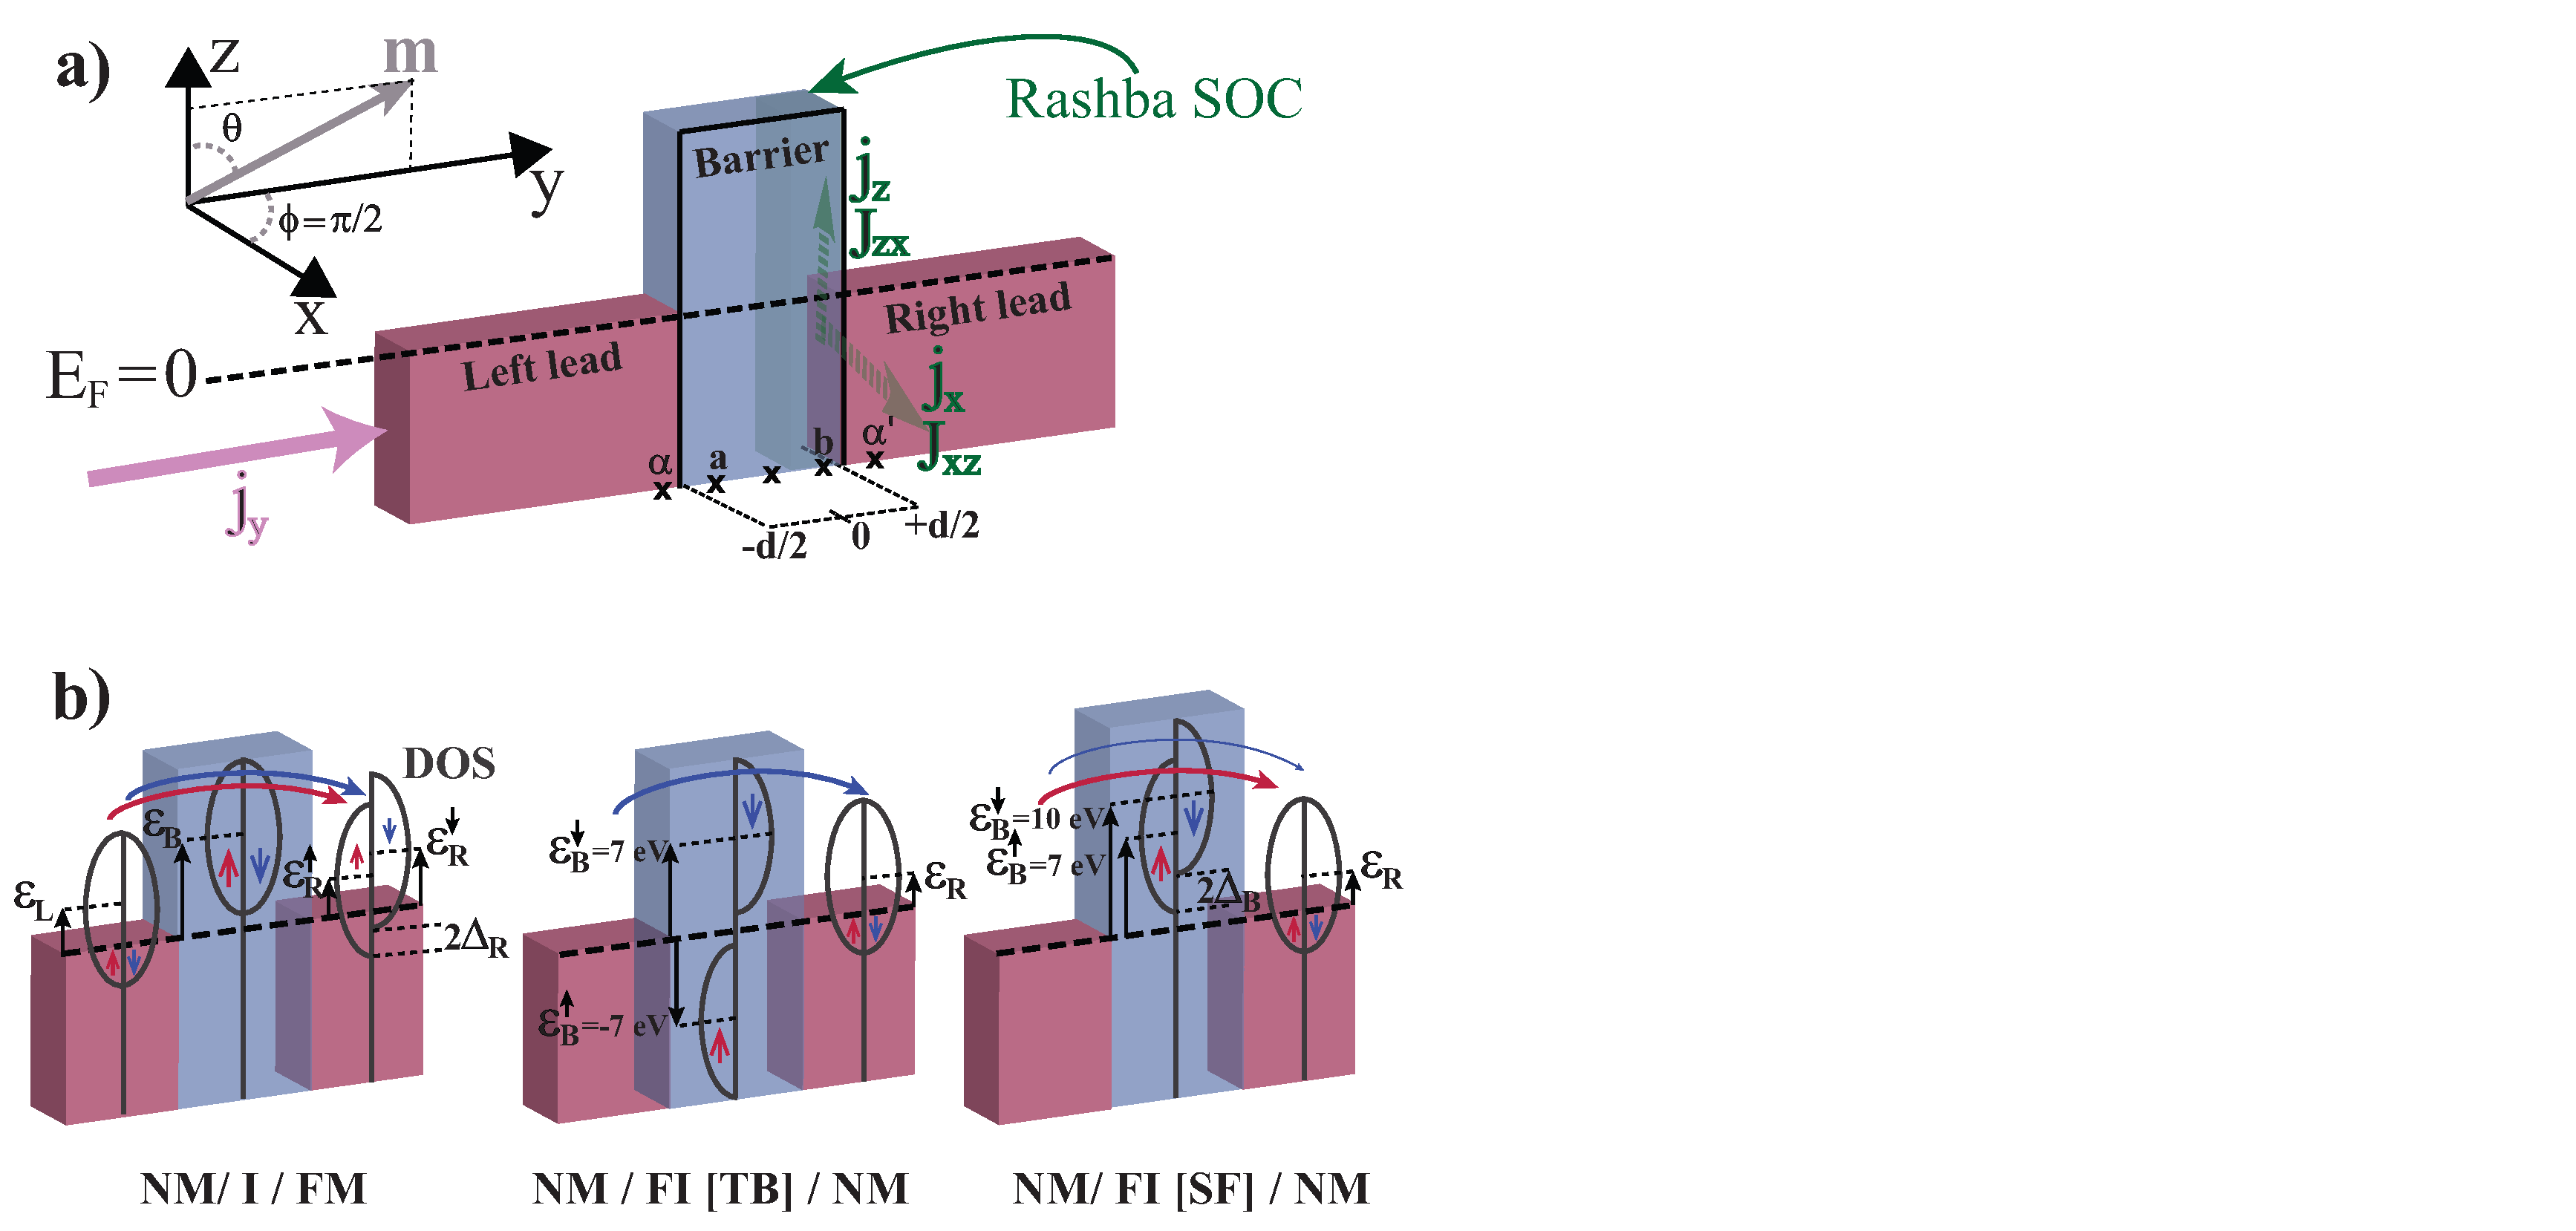
\includegraphics[width=1.85\columnwidth,clip=false]{fig1.eps}
\caption{(Online Color) a) Potential profile of a three-layers structure made of semi-infinite leads separated by a barrier region. The system is subjected to an interfacial Rashba SOC defined at position $y=b$ in the barrier (green color). It gives rise to the anomalous ($j_x, j_z$) and spin Hall ($J_{xz}, J_{zx}$) effects.  $E_{\tx{F}}$ is defined at zero, $\bm m$ is the magnetization vector in spherical coordinates, and $d$ is the barrier width. b) Tight-binding potential profile of systems made of non-magnetic and ferromagnetic barriers.  $\eps_{\Og}$ and $\Dlt_{\Og}$ are the on-site energy and exchange splitting in $\Og$ (\tx{L}, \tx{R}, or \tx{B}), respectively. Upperindex in $\eps^\sg$ refers to the spin orientation. In absence of $\sg= \upa$ or $\dna$, both contributions are equivalent. For the particular case of ferromagnetic barriers (FI), two sets of parameters with different density of states (DOS) are discussed. One represents the proper definition of a ferromagnetic insulator and is derived considering the single-band tight-binding, TB, Hamiltonian (center). The other is the free-electron spin filter, SF, approximation (right). The spin-dependent tunneling process is represented with blue and red arrows. Blue for spin-down and red for spin-up.}
\label{fig:figu1}
\end{figure}
%%%%%%%%%%%%%%%%%%%%%%%%%%
In this study, we investigate a three-layer structure comprising an insulating region sandwiched between two semi-infinite leads in two types of tunneling junctions: i) NM/I/FM and ii) NM/FI/NM, as shown in Fig.~\ref{fig:figu1}. Considering the tunneling current along the $y$-axis, the Hamiltonian of the free-electron model is expressed as the sum of the barrier potential:
\begin{equation}\label{eq:1}
H_{\rm B} =  \frac{\hbar^2 \bm k^2}{2m} + \Dlt_{\rm B}  \bm m_{\rm B} \cdot \bm \sg  + U(y) +  \lam (\bm y \times \bm k)\cdot  \bm \sg \mbox{ } \dlt \big(y- \frac{d}{2}\big).
\end{equation}
\noindent The Hamiltonian for the left and right leads is given by $H_{\rm L}= \frac{\hbar^2 \bm k^2}{2m}$ and $H_{\rm R} = \frac{\hbar^2 \bm k^2}{2m}+ \Delta_{\rm R}  \bm m_{\rm R} \cdot \bm \sigma$, respectively. In these expressions, the first term represents the kinetic energy with $\boldsymbol{k}$ being the wave-vector, $\hbar$ the Planck's constant, and $m$ is the effective electron mass. The second term involves the exchange interaction in the $s$-$d$ model \cite{Shubin1934}, where $\Delta_{\rm R}$ is the exchange splitting parameter, $\boldsymbol{\sigma}= (\sigma_{x},\sigma_{y},\sigma_{z})$ is the vector of Pauli matrices, and $\boldsymbol{m}_{\rm R} = (\cos\phi\sin\theta, \sin\phi\sin\theta,\cos\theta)$ is the magnetization vector given in spherical coordinates. In Eq.~(\ref{eq:1}), the third term corresponds to the barrier potential, and the last term is the Rashba spin-orbit coupling, where $\lambda$ is the Rashba parameter, and $d$ is the width of the barrier. The velocity operator due to Rashba SOC is given by $\bm v^{\rm so} = \frac{\lambda}{\hbar}(-\sigma_z,0,\sigma_x)$, indicating that the $x$$(z)-$component of the velocity reaches its maximum value when the magnetization vector of the ferromagnetic layer is aligned along the $z$$(x)-$axis. By symmetry arguments, one can expect the transverse current along $x$$(z)$ to exhibit a cosine (sine) behavoir as a function of $\theta$ when the magnetization vector is aligned within the $xz-$plane. Similarly, when the magnetization vector rotates in the $xy$ ($yz$)$-$plane, the transverse current along $z$ ($x$) is expected to display a cosine behavoir as a function of $\phi$ ($\theta$). Now, let us consider the spin current density, denoted as $J_{ij}$, where the subscripts $i$ and $j$ describe the spatial direction and spin orientation. For transport along $y$, Rashba SOC results in six components of the spin current density; however, physically only two components are real, with $J_{xz}$ = -$J_{zx}$. Unlike the anomalous charge current, the spin current is present even in the absence of a magnetic layer.


To gain a better understanding of these spin-orbit effects, we initially solve the quantum transport across the sample within the free electron picture. In this approach, any observable stems from the contributions of electrons flowing from the left lead (L) to the right lead (R) and vice versa. This approximation has been widely employed in tunnel junctions, not only for describing symmetric filtering in magnetic tunnel junctions but also for elucidating the spin filtering process in ferromagnetic barriers \cite{sf, Eu}. In the latter system, conventionally, two spin channels, majority and minority, are considered, with an exchange splitting above the Fermi level leading to a spin-dependent tunneling process dominated by the majority carriers (see Fig. \ref{fig:figu1}(b), right). However, when studying ferromagnetic insulators, the limitation of this approach arises because the magnetic order is not well defined. In the subsequent section, a proper definition is provided by considering the tight-binding model. In this case, the density of states of majority carriers, responsible for the magnetic order in the insulator, is fully occupied below the Fermi level. Consequently, only the minority spin channel contributes to the tunneling process (see Fig. \ref{fig:figu1}(b), center). To achieve a similar description using the free electron approximation, one needs to neglect the contribution of one spin channel. Therefore, for qualitative agreement with the tight-binding Hamiltonian, in this section, we begin by considering two spin channels above the Fermi level and take into account a large exchange splitting to disregard the upper band. Our initial focus is on studying the anomalous and spin Hall effects. To the lowest order in the barrier transmission, we have:
\begin{equation}
\begin{aligned}
\bm j^{\rm so} = \frac{e\lam}{\hbar}  \bm j_{\rm R\raw L}^{\rm so},~~~~ \bm J^{\rm so} = \frac{\lam}{2} \bm J_{\rm R\raw L}^{\rm so}, 
\label{Jso}
\end{aligned}
\end{equation}
where $\bm j^{\rm so}=(j_x^{\rm so},j_z^{\rm so})$ and $\bm J^{\rm so} = (J^{\rm so}_{xz},J^{\rm so}_{zx})$  are, respectively, the anomalous and spin Hall current density pairs. Eq. \eqref{Jso} implies that AHE and SHE in tunnel junctions are interfacial effects driven by electrons flowing from right to left (${\rm R \raw L}$). In simpler terms, the contribution of tunneling electrons (${\rm L \rightarrow R}$) is negligible as it is determined at a higher order in the barrier transmission. Consequently, we restrict our study to bilayer systems of the form FI/NM and I/FM. At zeroth order in the barrier transmission, we have:
\begin{align}
\label{jxxooo}
 \bm j^{\rm so, \tx{FM}} &= 2\lam\xi\frac{\dlt_k(k_{\rm R}^\dna k_{\rm R}^\upa - q_{\rm R}^2)}{D_{k}} (\cos \theta_{\rm R}, -\sin \theta_{\rm R}\cos \phi_{\rm R}), \\
\label{jzzooo}
\bm j^{\rm so, \tx{FI}} &= 2\lam\xi\frac{ \dlt_q \Sg_q k_{\rm R}}{D_{q}}(\cos \theta_{\rm B}, -\sin \theta_{\rm B}\cos\phi_{\rm B}), \\
\label{Jxz00}
\bm J^{\rm so, \tx{FM}} &= \left [ \lam \frac{ \Sg_k (k_{\rm R}^\dna k_{\rm R}^\upa + q_{\rm R}^2)}{D_k}  + \lam^3\mathcal{G}^{\text{FM}}_{(\phi_{R},\theta_{R})} \right] (1, -1),\\
\bm J^{\rm so, \tx{FI}} &=   \left [ \lam\frac{ k_{\rm R} (2k_{\rm R}^2 + q_{\rm R}^{\upa 2} + q_{\rm R}^{\dna 2})}{D_q} + \lam^3\mathcal{G}^{\text{FI}}_{(\phi_{B},\theta_{B})}\right] (1, -1). 
 \label{Jxz002}
\end{align}
In the provided expressions, the superscript FM (FI) denotes the system I/FM (FI/NM). Furthermore, $\xi = e/\hbar$, $D_{k}=(k_{\rm R}^{\downarrow 2} + q_{\rm R}^{2})(k_{\rm R}^{\uparrow 2} + q_{\rm R}^{2})$, $D_{q} = (k_{\rm R}^2 + q_{\rm R}^{\downarrow 2})(k_{\rm R}^2 + q_{\rm R}^{\uparrow 2})$, $\Sigma_q(\delta_q) = q_{\rm R}^{\downarrow} \pm q_{\rm R}^{\uparrow}$, and $\Sigma_k(\delta_k)=k_{\rm R}^{\downarrow} \pm k_{\rm R}^{\uparrow}$. Here, $k_{\rm R}$ is the right lead wave-vector, and $q_{\rm R}$ is the barrier wave-vector at the right interface. Eqs.~ \eqref{jxxooo} and \eqref{jzzooo} describe the anomalous Hall current density, where $|\bm j^{\rm so}|$ is independent of the magnetization orientation when the angle spanned by the magnetic vector lies in the $xz-$plane. As indicated, the $x$$(z)-$component of the anomalous Hall effect exhibits a cosine(sine) dependence as a function of $\theta$. In the absence of the exchange splitting, either in the insulating barrier ($\delta_q = 0$) or the lead ($\delta_k = 0$), the anomalous Hall effect vanishes. In contrast, the spin Hall current density, given in Eqs.~\eqref{Jxz00} and \eqref{Jxz002}, is nonzero in the absence of the exchange splitting. It is important to note that this result acquires an angular dependence, denoted by the function $\mathcal{G}$, when considering higher orders of $\lambda$. To introduce an angular dependence to the first order in Rashba SOC, FI/FM bilayers are necessary, as discussed in Ref. \onlinecite{fifm}.


An intriguing observation is that the anomalous Hall current density is nonzero at zero bias. This was previously highlighted in Ref. \onlinecite{vedyayev_prl}, where the authors considered spin-orbit coupled impurities in the insulating region of a magnetic tunnel junction. The underlying reason lies in the electric field that generates the Rashba term. If this field is induced by the effective potential drop across the junction, then in the absence of bias, we have  $\lambda = 0$. However, if this field is material-dependent and is driven by the broken inversion symmetry at the interface of two samples, it results in an effective current that spontaneously diffuses in the absence of bias until reaching a steady state. In the presence of applied bias, Eqs. \eqref{jxxooo} and \eqref{jzzooo} remain dominant, serving as the basis for a comprehensive understanding of the anomalous Hall effect.

A noteworthy feature from Eqs. \eqref{jxxooo} to \eqref{Jxz002} is that the amplitudes of the anomalous and spin Hall current densities do not exhibit significant differences when considering a ferromagnetic insulator or a ferromagnetic lead. This is attributed to the negligible contribution of tunneling electrons. Next, we proceed to the discussion of tunneling anisotropic magnetoresistance (TAMR), extensively studied in Ref. \onlinecite{tamr0} for semi-magnetic tunnel junctions of the form NM/I/FM. In this work, we compare this system with the case of normal metal leads attached to a ferromagnetic insulator, i.e., NM/FI/NM. In the presence of Rashba SOC, the tunneling current density, $j_y$, for electrons flowing from ${\rm R \rightarrow L}$, exhibits the general form:
\begin{align}
j_{y,{\rm R\raw L}}^{\tx{FM}(\tx{FI})}(\phi_{\rm R (B)},\theta_{\rm R (B)}) \propto  1 + \lam^2 k^2_\para \mathcal{F}^{\tx{FM}(\tx{FI})}_{(\phi_{\rm R (B)},\theta_{\rm R (B)})}.
\label{jy9}
\end{align}
In Eq.~ \eqref{jy9}, the angular integration over $\bm k_\parallel$ has been conducted (with $|\bm k_\parallel| = k_\parallel$). The same expression is obtained at zero bias for electrons flowing from left to right. In contrast to the anomalous Hall effect, the angular dependence of the tunneling current, characterized by the function $\mathcal{F}$, emerges at the second order in Rashba SOC. Additionally, when the magnetic vector rotates within the $xz-$plane ($\phi = 0$), the anisotropy is zero, regardless of whether ferromagnetic leads or ferromagnetic insulators are considered. For rotations along the $xy-$ and $yz-$planes, the tunneling anisotropic magnetoresistance is given by:
% i.e., $\Dlt \bm j_{R\raw L[xz]}^{\tx{FM} (\tx{FI})} = \bm j_{R\raw L}^{\tx{FM}(\tx{FI})}(0,\theta_{R (B)}) - \bm j_{R\raw L}^{\tx{FM} (\tx{FI})}(0,0) = 0.$ 
\begin{align}
\label{tamr1}
\tx{TAMR}^{\tx{FM}(\tx{FI})}_{[xy]} &= \frac{\Dlt j^{\tx{FM}(\tx{FI})}_{y,[xy]}}{j_y^{\tx{FM}  (\tx{FI})}(\phi_{\rm R (B)},\pi/2) }, \\
\tx{TAMR}^{\tx{FM}(\tx{FI})}_{[yz]} &= \frac{\Dlt j^{\tx{FM}(\tx{FI})}_{y,[yz]}}{j_y^{\tx{FM}  (\tx{FI})}(\pi/2,\theta_{\rm R (B)}) },
\label{tamr2}
\end{align}
where 
\begin{subequations}
\begin{equation}
\Dlt j^{\tx{FM}(\tx{FI})}_{y,[xy]} = j_y^{\tx{FM}  (\tx{FI})}(0,\pi/2) - j_y^{\tx{FM}  (\tx{FI})}(\phi_{\rm R (B)},\pi/2)
\end{equation}
and 
\begin{equation}
\Dlt j^{\tx{FM}(\tx{FI})}_{y,[yz]} =  j_y^{\tx{FM}  (\tx{FI})}(\pi/2,0) -  j_y^{\tx{FM}  (\tx{FI})}(\pi/2,\theta_{\rm R (B)}),
\end{equation}
\end{subequations}
such that $ j_y^{\tx{FM}  (\tx{FI})}(\phi_{R (B)},\theta_{R(B)})$ is the total current given by the contributions of electrons flowing from left to right and vice-versa. In particular, from right to left, we obtain
\begin{align}
\frac{\tx{TAMR}_{R \raw L[xy(yz)]}^{\tx{FM}} }{ \tx{TAMR}_{R \raw L[xy(yz)]}^{\tx{FI}}} \approx \frac{ \Dlt_{\rm R}^2 D_q^2 \beta_0 }{ \Dlt_{\rm B} D_k^2 \beta_0^*}.
\label{ratiotamr}
\end{align}
where $\beta_0 (\beta_0^*)$ is defined in Ref. \onlinecite{atmr}. Eq.~ \eqref{ratiotamr} provides a simplified perspective for understanding the distinctions between employing a ferromagnetic insulator or a ferromagnetic lead in the investigation of tunneling anisotropic magnetoresistance. It suggests a more pronounced dependence on the exchange splitting rate when a ferromagnetic lead is considered, a feature that will be observed in the subsequent section on our numerical calculations. The third aspect to address is the Rashba-induced spin-orbit torque. As highlighted in Ref. \onlinecite{sot}, Rashba SOC acts as a source for the spin density, consequently leading to the generation of a spin torque of the form $\bm T^{\text{FM} (\text{FI})} = \frac{2\Delta_{\rm R (B)}}{\hbar} \bm S \times \bm m_{\rm R (B)}$ within the magnetic layer. Here, $\bm T$ represents the spin torque applied to $\bm m$, and $\bm S$ is the spin density.
%In spherical coordinates we have $\bm T = T_\theta \bm{\h e}_\theta + T_\phi \bm{\h e}_\phi,$ which offers a more general definition of the Rashba torque than the conventional in-plane, $T_\para$, and out-of-plane, $T_{\perp}$, components \cite{pauyacapl}. 
When the magnetization undergoes rotation within the plane of the Rashba SOC ($xz-$plane), $\bm T = 0$; hence, no spin torque is anticipated under these conditions. For rotations along the $xy-$ and $yz-$planes, the expressions are as follows:
\begin{align}
\label{deft1}
\bm T_{[xy]}^{\tx{FM}(\tx{FI})} &=   \frac{2\Dlt_{\rm R (B)}}{\hbar} (S_x \sin \phi_{\rm R(B)} - S_y \cos \phi_{\rm R(B)}) ~\bm{\h k}, \\
\bm T_{[yz]}^{\tx{FM}(\tx{FI})} &=  \frac{2\Dlt_{\rm R (B)}}{\hbar} (S_y \cos \theta_{\rm R(B)} - S_z \sin \theta_{\rm R(B)}) ~\bm{\h i},
\label{deft2}
\end{align}
where $\bm{\h i}$ and $\bm{\h k}$ represents the unit vectors along the $x$ and $z$ axes. Eqs.~ \eqref{deft1} and \eqref{deft2} are conventionally known as the out-of-plane components of the Rashba torque ($T_\perp$), because, their orientation is perpendicular to the plane defined by the transport direction and the magnetization orientation. Generally, the Rashba torque can be divided into two components, $T_\perp$ and $T_\parallel$. The latter, known as the in-plane component, is omitted in this report due to its significantly smaller magnitude compared to the net out-of-plane component, i.e., $T_\parallel(V) \ll T_{\perp}(V) - T_{\perp} (V=0),$ where $V$ represents the voltage drop. At zeroth order in the barrier transmission and second order in Rashba SOC, the out-of-plane component is given by:
\begin{align}
\label{torqu1}
T_{\rm R \raw L [xy(yz)]}^{\tx{FM}} &= \mp \gamma_{\rm R} \frac{ \dlt_k  [(k_{\rm R}^{\dna} k_{\rm R}^{\upa} - q_{\rm R}^2)^2 -\Sg_k^2q_{\rm R}^2]}{D_k^2}\sin 2\phi(\theta)_{\rm R},\\
T_{\rm R \raw L [xy(yz)]}^{\tx{FI}} &= \mp 2\gamma_{\rm B} \frac{  \dlt_q \Sg_q  k_{\rm R}( k_{\rm R}^2 - q_{\rm R}^\dna q_{\rm R}^\upa)}{D_q^2}\sin 2\phi(\theta)_{\rm B} , 
\label{torqu2}
\end{align}
with $\gamma_{R(B)} = 8 m^2 \pi \Dlt_{R(B)}\lambda^2  k_\para^2 / \hbar^4$. Eqs.~ \eqref{torqu1} and \eqref{torqu2} represent the local spin torques obtained at the right interface ($y = d/2$) for electrons flowing from right to left. The contributions from electrons flowing in the opposite direction are given at a higher order; hence, the aforementioned expressions serve as the foundation for a comprehensive understanding of the Rashba torque. Notably, whether considering a ferromagnetic lead or a ferromagnetic insulator, the Rashba torque exhibits an angular dependence in the form of $\sin2\theta(\phi)$. Furthermore, these outcomes remain independent of the barrier transmission, indicating that the Rashba torque is an interfacial effect predominantly influenced by electrons flowing from right to left.

In this section, we have derived analytical expressions based on the free electron model to address the angular dependence of Rashba-induced spin-orbit effects in tunnel junctions with the presence of a ferromagnetic insulator or a ferromagnetic lead, i.e., NM/(FI/NM and I/FM). These expressions suggest that interfacial spin-orbit effects driven by electrons flowing from right to left, such as the Rashba torque and the anomalous and spin Hall effects, do not exhibit significant differences between FI/NM and I/FM structures. However, when the contribution of tunneling electrons is no longer negligible, specific differences emerge, as indicated in Eq.~ \eqref{ratiotamr} when investigating the tunneling anisotropic magnetoresistance. It is important to note that these results are presented at zero bias and to the lowest order in Rashba and barrier transmission. The subsequent section will involve a thorough analysis of these spin-orbit effects, presenting numerical findings in the non-equilibrium regime.


%%%%%%%%%%%%%%
%%%%%%%%%%%%%
\section{Numerical results}\label{sec:sec2}
In this section, we employ the simple cubic tight-binding Hamiltonian within the Keldysh formalism. To maintain clarity in our analysis while capturing essential physics, detailed analytical derivations are provided in the supplementary material, as we focus on key equations. It is important to highlight that, unlike the free electron model discussed in the preceding section, the Rashba Hamiltonian is defined within the barrier region, as depicted in Fig. \ref{fig:figu1}(b). Consequently, the one-electron Schr\"odinger's equation for the spin-dependent isolated Green's function is expressed as
\begin{widetext}
\begin{equation}
\sum_{p_1} \Bigg \{ \bigg\{ [(E-\eps_{\bm{k}_{||}})\dlt_{pp_1}-\overline{H}_{pp_1}]\hat{I}-\dlt H_{p,p_1} \bigg[\begin{array}{ccc}\cos\theta_\Og & \sin\theta_\Og e^{-i\phi_\Og} \\
\sin\theta_\Og e^{i\phi_\Og} & -\cos\theta_\Og 
 \end{array} \bigg] -  \bar{\lambda} \left(\begin{array}{cc} 
2\sin k_xa  &  -2\sin k_za\\
-2\sin k_za &  -2\sin k_xa
\end{array}\right) \bigg \} \left(\begin{array}{cc} \hat{g}^{\upa\upa}_{p_1q}  &  \hat{g}^{\upa\dna}_{p_1q} \\  \hat{g}^{\dna\upa}_{p_1q} &  \hat{g}^{\dna\dna}_{p_1q} \end{array}\right)  \Bigg \}=\dlt_{pq}\hat{I},
 \label{tbschrodinger}
\end{equation}
\end{widetext} 
where $p_1$, $p$, and $q$ represent atomic sites along the $y$-axis. $E$ is the total energy, and $\eps_{\bm k_\para} = 2t(\cos k_x a + \cos k_z a)$ is the in-plane component of the energy, where $a$ is the lattice constant, and $t$ is the hopping matrix element. Furthermore,  $\overline{H}_{pq} = \eps^0_\Omega\delta_{pq} + t(\delta_{p,q+1}+\delta_{p,q-1})$ and $\delta H_{pq}= \Delta_\Omega \delta_{pq}$, 
where $\eps^0$ and $\Dlt$ are the on-site energy and exchange splitting parameters, respectively.  $\Omega$ represents the left (L), right (R), or barrier (B) region. In this study, $\Delta_L = 0$, and the magnetization vectors in $R$ and $B$ are defined in spherical coordinates with angles $\theta$ and $\phi$. The third term is the Rashba matrix in the nearest neighbor approximation, where $\bar{\lambda} = \frac{\lambda}{2a}\delta_{p_1b}$ represents the effective Rashba parameter, and $p_1=b$ denotes the barrier site adjacent to the right lead. $\hat{G}$ is the $2\times2$ isolated Green's function matrix, and $\hat{I}$ is the $2\times2$ unit matrix operator. 


Equation \eqref{tbschrodinger} is solved by means of the matrix inversion in the barrier and Dyson's equation in the semi-infinite leads. To obtain the isolated retarded (advanced) Green's functions, we consider $E \rightarrow E \pm i\delta$, where $\delta$ is an infinitesimal value. Subsequently, we proceed to couple the system composed of semi-infinite leads attached to the barrier. We obtain,
\begin{align}
\h G_{pq}^{r(a)} = \h g_{pq}^{r(a)} + \h g_{pa}^{r(a)} \h \Sg_{L}^{r(a)} \h G_{aq}^{r(a)} + \h g_{pb}^{r(a)} \h \Sg_{R}^{r(a)} \h G_{bq}^{r(a)},
\label{eq:G}
\end{align}
where $\hat{G} (\hat{g})$ is the $2\times2$ coupled (isolated) Green's function matrix, where the superscripts $r(a)$ indicate retarded (advanced), and subscripts $a(b)$ correspond to the atomic site next to the left (right) interface. The terms $\hat{\Sigma}^{r(a)}_{L} = t^2 \hat{g}^{r(a)}_{\alpha\alpha}$ and $\hat{\Sigma}^{r(a)}_{R} = t^2 \hat{g}^{r(a)}_{\alpha'\alpha'}$ are known as the self-energy terms, describing the electron's propagation across the left and right interfaces, respectively. The subscripts $\alpha (\alpha')$ refer to the left (right) lead atomic site adjacent to the barrier. To analyze the system under an external bias, non-equilibrium Green's functions are employed. In the Keldysh formalism, the quantum kinetic equation reads
 \begin{align}
 \label{fullself5}
 \h G^<_{pq} = \h g^<_{pq} &+ t (\h G^<_{L } +  \h G^<_{R }),
 \end{align}
 such that, $\h G^<_{pq} (\h g^<_{pq})$ is the $2\times2$ coupled(isolated) lesser Green's function matrix, where $\h{G}^<_L = \h g^r_{p\alp}\h G^<_{aq} + \h g^r_{pa} \h G^<_{\alp q} +  \h g^<_{p\alp} \h{G}^a_{aq} + \h g^<_{pa}\h{G}^a_{\alp q}$  and $\h{G}^<_{\rm R}  = \h g^r_{pb}\h G^<_{\alp' q} + \h g^r_{p\alp'}\h G^<_{bq} +  \h g^<_{pb} \h{G}^a_{\alp' q} + \h g^<_{p\alp'}\h{G}^a_{bq}$ denote the contributions of the electrons from the left and from the right, respectively.  To study the spin-orbit effects discussed in the previous section, Eq. \eqref{fullself5} is employed, as it gives a direct link between the density matrix and any physical quantity in the non-equilibrium regime. First, we examine the tunneling anisotropic magnetoresistance, where we evaluate the tunneling current density in the mixed representation using the expression: 
\begin{align}
\langle j_y \rangle &=  \tx{Re} \sum_\sg  \bigg{[} \frac{\xi t}{8\pi^3} \int \Big{(}   \h G_{j+1,j}^{\sg\sg <}  - \h G_{j,j+1}^{\sg\sg <} \Big{)} dE d\bm k _\para \bigg{]}, 
\label{qchargeoky}
\end{align}
and employ the definitions provided in Eqs. \eqref{tamr1} and \eqref{tamr2}. Following this, we investigate the anomalous and spin Hall effects, decomposing the total current density into two components, i.e., $j_{x(z)} = j^n_{x(z)} + j^{\rm so}_{x(z)}$ and $J_{xz} = J_{xz}^n + J_{xz}^{\rm so}$. The first component represents the normal current driven by the kinetic contribution, while the second arises in the presence of SOC. In the preceding section, only the second component was examined, as shown in Eqs. \eqref{jxxooo}-\eqref{Jxz002}. In this context, the two components are expressed as
\begin{align}
\langle j_{x}^n \rangle &= \tx{Re} \sum_{j,\sg} \bigg{[}i\frac{\xi t}{4\pi^3}\int  \h G^{\sg,\sg <}_{j,j} \sin k_{x} dE d\bm k _\para \bigg{]}, \\
\langle j_{z}^n \rangle &= \tx{Re} \sum_{j,\sg} \bigg{[}i\frac{\xi t}{4\pi^3}\int  \h G^{\sg,\sg <}_{j,j} \sin k_{z} dE d\bm k _\para \bigg{]}, \\
\langle J_{xz}^n \rangle &= \tx{Re} \sum_{j,\sg} \bigg{[}  i\frac{t}{8\pi^3}\int    \sg \h G_{jj}^{\sg\sg <}  \sin k_x   dE d\bm k_\para  \bigg{]}, 
\end{align}
and
\begin{align}
\langle j_x^{\rm so} \rangle &=  \tx{Re} \sum_{j, \sg} \bigg{[} i\frac{\xi\bar{\lam}}{4\pi^3} \int  \sg^* \h G^{\sg,\sg <}_{j,j} \cos k_x   dE d\bm k _\para \bigg{]}, \\
\langle j_z^{\rm so} \rangle &= \tx{Re}  \sum_{j,\sg} \bigg{[}i\frac{\xi\bar{\lam}}{4\pi^3} \int  \h G^{\sg,\sg^* <}_{j,j} \cos k_z  dE d\bm k _\para \bigg{]}, \\
\langle J_{xz}^{\rm so} \rangle &= \tx{Re} \sum_{j,\sg} \bigg{[} i\frac{\bar{\lam}}{8\pi^3}  \int  \h G_{jj}^{\sg\sg <}  \cos k_x dE d\bm k_\para \bigg{]}. 
\end{align}
Finally, we address the Rashba torque by examining the components of the spin density,
\begin{align}
\langle S_x \rangle &= \tx{Re}\bigg{[}\frac{\hbar}{16\pi^3i}  \sum_{j,\sg} \int  \h G_{jj}^{< \sg \sg^*} dE d\bm k _\para\bigg{]}, \\
\langle S_y \rangle &= \tx{Re}\bigg{[}\frac{\hbar}{16\pi^3}  \sum_{j,\sg} \int  \sg \h G_{jj}^{< \sg \sg^*} dE d\bm k _\para\bigg{]}, \\
\langle S_z \rangle &= \tx{Re}\bigg{[}\frac{\hbar}{16\pi^3i}  \sum_{j,\sg} \int \sg \h G_{jj}^{< \sg \sg} dE d\bm k _\para\bigg{]},
\end{align}
and employ the expressions provided in Eqs. \eqref{deft1} and \eqref{deft2}. 
In the above formulations, $\sigma = \uparrow (+)$ or $\downarrow (-)$ denotes spin-up or spin-down, $\sigma^*$ represents the opposite of $\sigma$, and the subscript $j$ indicates the atomic site in the barrier. It is noteworthy that all quantities have undergone Fourier transformation, capitalizing on the translational invariance along the $xz-$plane. This study employs two sets of tight-binding parameters to characterize ferromagnetic insulators. The first set is based on the conventional free-electron spin filter (SF) approximation, considering two spin channels exchange-split above the Fermi level, as utilized in the preceding section to derive analytical expressions. The second set of parameters defines a ferromagnetic barrier according to the single-band tight-binding (TB) Hamiltonian. This model assumes that the density of states of majority carriers is entirely occupied below the Fermi level, leading to a tunneling process dominated by the minority spin band, as depicted in Fig. \ref{fig:figu1}(b), center. In the subsequent discussions, FI-structures will be denoted as FI [SF] or FI [TB] depending on the parameters used. 
%Additional insights are provided towards the end when considering first principles calculations.

The analysis begins with the investigation of tunneling anisotropic magnetoresistance, presented in Fig. \ref{fig:figu2}, main panel, as a function of $\delta$. FI [SF] and FI [TB] are set with $\delta = (\epsilon_B^\downarrow - 7)$ eV. FM is set with $\delta = (\epsilon^\downarrow - 1)$ eV. In all cases, the majority spin-band is fixed and therefore $\delta$ becomes proportional to the exchange splitting.
In particular, in FI structures,  $\delta$ signifies the barrier height of the minority band above the Fermi level. Other parameters are detailed in the caption of Fig. \ref{fig:figu2}, where the leads correspond to materials without polarization inversion and have previously replicated experimental measurements in magnetic tunnel junctions \cite{kalitsov}. The focus is on rotations of the magnetic vector along the $yz$-plane.
\begin{figure}
\centering
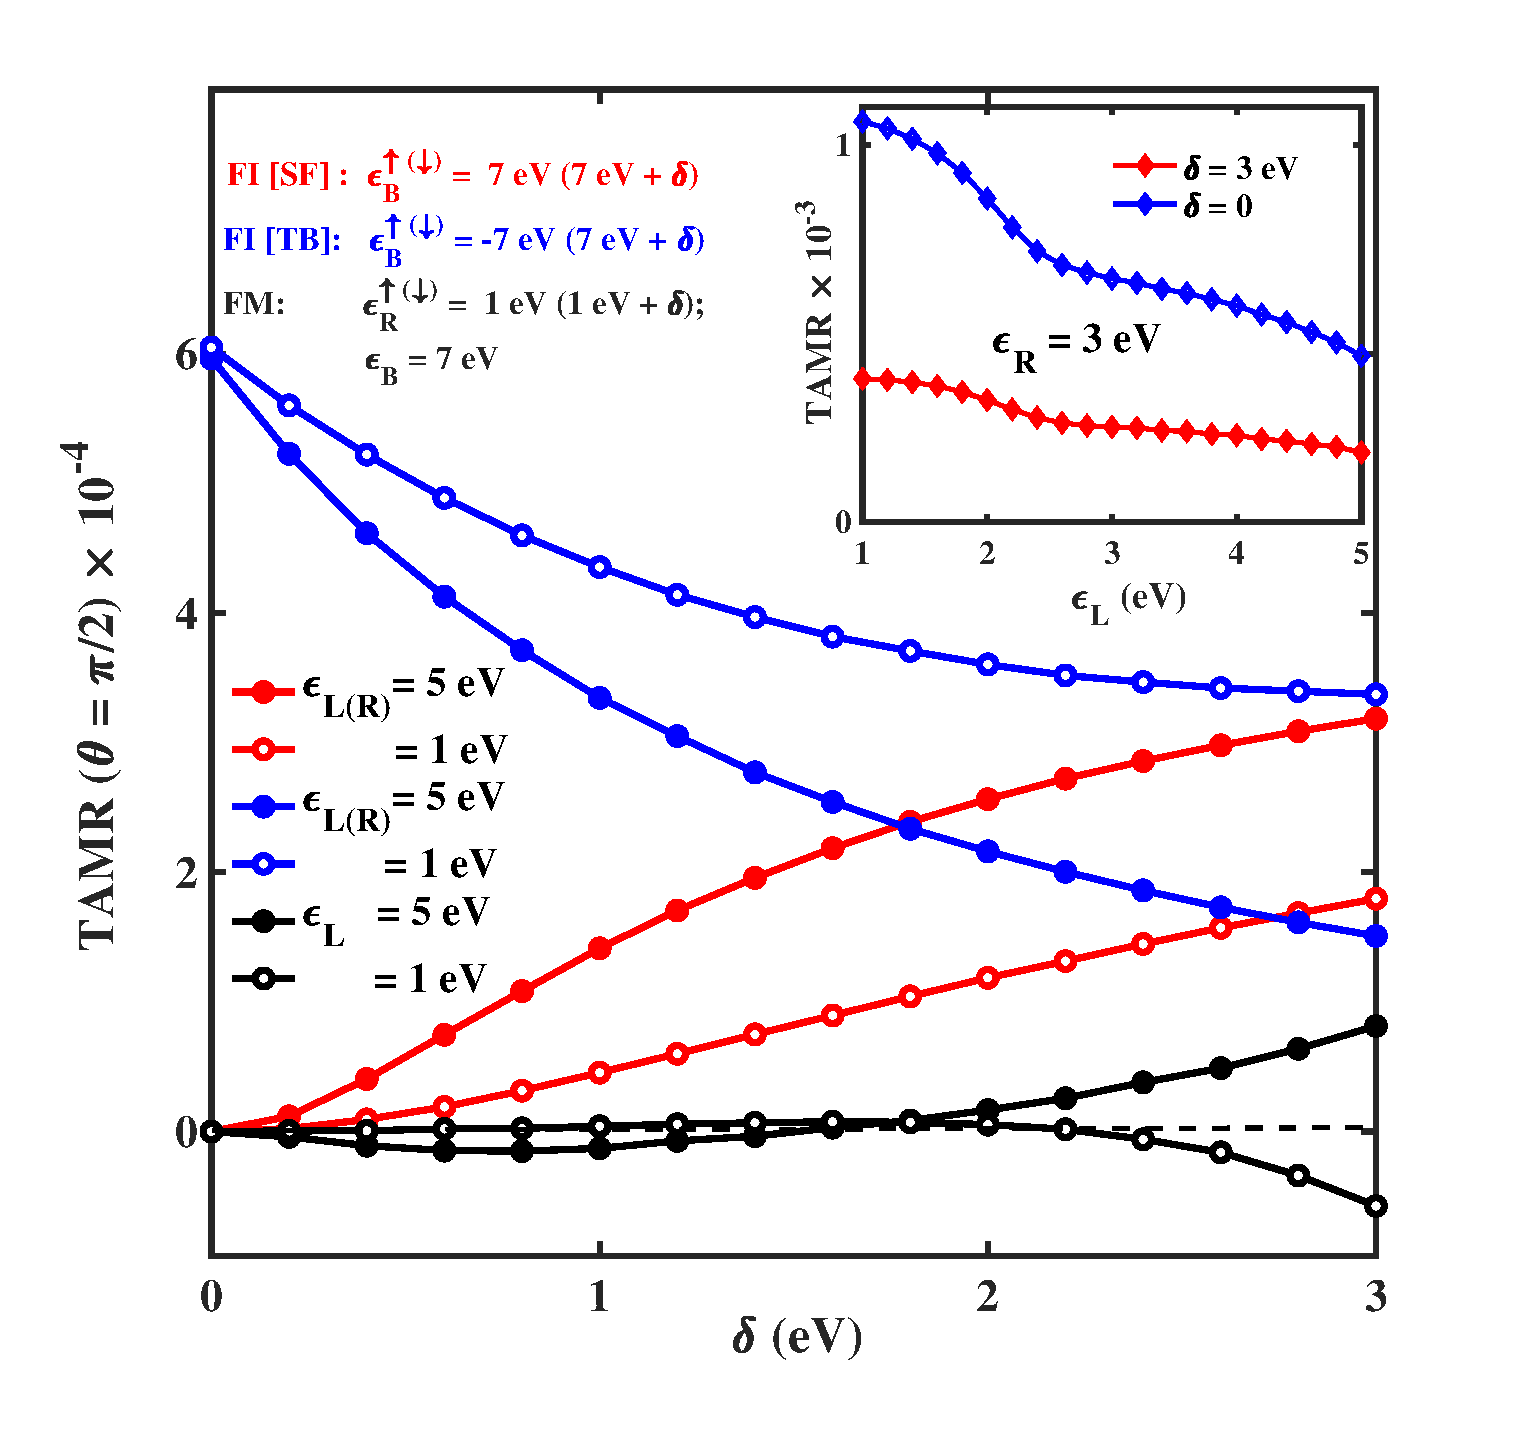
\includegraphics[width=1.0\columnwidth,clip=false]{fig2.eps}
\caption{(Online Color) $\text{TAMR}_{[\text{yz}]}$ ($\theta = \pi/2$), according to Eq. \eqref{tamr2}, as a function of  $\delta$ (main panel) and $\eps_L$ (inset) for FM and FI. Ferromagnetic insulators are represented with two sets of parameters: free-electron spin filter (SF) and  single-band tight-binding (TB). In all cases, the normal metal leads take two values, $\eps= 5$ eV (closed symbols) and $\eps= 1$ eV (open symbols). $\delta$ is proportional to the exchange splitting. In FI, $\delta =(\eps^\downarrow_B - 7)$ eV. In FM,  $\delta =(\eps^\downarrow_R - 1)$ eV. In the inset, asymmetric leads for ferromagnetic insulators are considered. The voltage drop is set to $V = 0.5$ eV. $t=1.0$ eV and $\lam = 0.05$ eV.}
\label{fig:figu2}
\end{figure}
In Eq. \eqref{ratiotamr} we showed that TAMR in the presence of ferromagnetic leads exhibits a more pronounced dependence on the exchange splitting rate in contrast to ferromagnetic insulators. This is in agreement with our numerical results, given in Fig. \ref{fig:figu2}. When comparing FM and FI [SF], the tunneling anisotropic magnetoresistance exhibits a quadratic dependence on the exchange splitting in the presence of ferromagnetic leads (black lines), while in the presence of ferromagnetic insulators, it displays a linear contribution to the exchange that becomes more pronounce as we populate the density of states in the leads (red open circles). Notably, FI [TB], in contrast to FI [SF], yields TAMR amplitudes that decrease with increasing $\delta$. This occurs because in the TB model, where only one spin band is considered for the tunneling process, an increase in $\delta$ corresponds to a higher barrier height. In the SF model, where both majority and minority bands exist above the Fermi level, an increase in $\delta$ primarily raises the barrier height for minority carriers, leading to an enhanced tunneling process for spin-up electrons.

An important feature when considering structures with similar barrier heights is that TAMR in FI/NM structures can be an order of magnitude larger than in I/FM structures, refer to Fig \ref{fig:figu2}. This suggests potential advantages for realizing anisotropic sensors and memory functionalities in tunneling devices. This result aligns with experimental findings, where ferromagnetic metals in the low band filling regime exhibit TAMR percentages below 3\%, whereas ferromagnetic insulators achieve TAMR amplitudes of 30\% or higher. Moreover, unlike I/FM structures, where the amplitude changes sign when tuning the band filling in the leads or the exchange splitting in the ferromagnetic layer, FI/NM structures do not show sign reversal due to the spin filtering process in the ferromagnetic barrier. The inset in Fig. \ref{fig:figu2} illustrates the role of the asymmetry in FI/NM structures. The amplitude of TAMR increases as the density of states in the left lead is populated. In I/FM systems, on the other hand, sign reversal is evident in asymmetric junctions (black lines in Fig. \ref{fig:figu2} main panel).
\begin{figure}
\centering
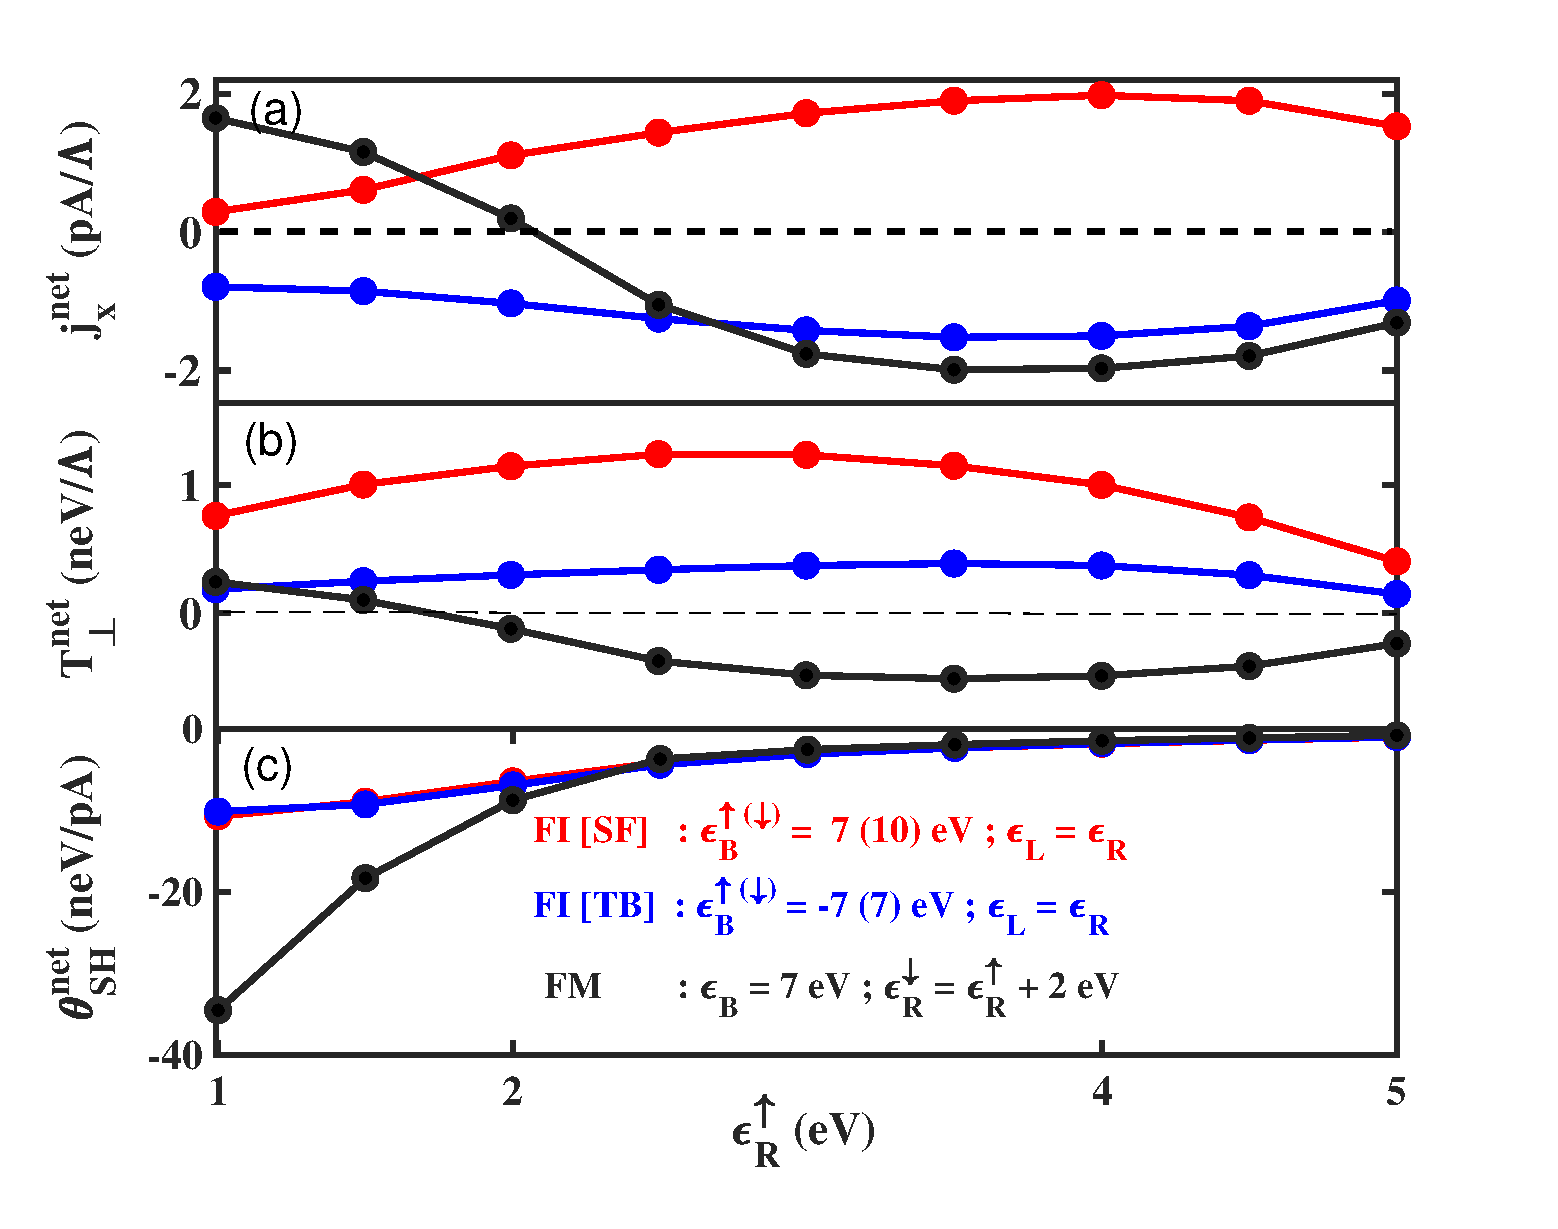
\includegraphics[width=0.8\columnwidth,clip=false]{fig3.eps}
\caption{(Online Color) The anomalous Hall effect, the Rashba torque, and the spin Hall angle as a function of the on-site energy in the right lead ($\eps^\upa_{\rm R}$) for a fixed magnetization orientation along the $yz-$plane ($\theta = \pi/4$ for the Rashba torque, and $\theta = 0$ for the anomalous Hall effect and the spin Hall angle). In all cases, the contribution at zero bias is subtracted and therefore we use the upperindex \textit{net}. $\eps_L = \eps_{\rm R}^\upa$, $V = 0.5$ eV, $t = 1.0$ eV, and $\lambda = 0.05$ eV. Other parameters are given in the legend of the figure.}
\label{fig:figu3}
\end{figure}

Next, we delve into the discussion of the Rashba torque, anomalous and spin Hall effects, depicted in Fig. \ref{fig:figu3}, focusing on the on-site energy in the right lead. Specifically, for the spin Hall effect, we analyze the spin Hall angle, denoted as $\theta^{\text{net}}_{SH} = J^{\text{net}}_{xz}/j_y$. In all cases, the maximum values are considered with the magnetic vector oriented along the $yz$-plane ($\theta = \pi/4$ for the Rashba torque and $\theta = 0$ for the anomalous and spin Hall effects). The contribution at zero bias is subtracted, denoted by the upper index \textit{net}. It's important to note that variations in $\eps_L$ won't contribute significantly to these spin-orbit effects [see Eq. \eqref{Jso}]. The left lead is held constant relative to the right lead ($\eps_L = \eps_{\rm R}^\upa$).
For equivalent exchange values, the Rashba torque and the anomalous Hall effect exhibit similar amplitudes for both types of systems, as shown in of Fig. \ref{fig:figu3} (a). In the case of a ferromagnetic insulator, they become robust against sign reversal. Conversely, when considering a ferromagnetic lead, the amplitudes change sign as the system transitions from the half-metallic to the low band-filling regime. This is a consequence of the Slonczewski polarization present in magnetic tunnel junctions \cite{cop}.

An interesting observation in ferromagnetic insulators is that the amplitudes of the Rashba torque exhibit the same sign for SF and TB, while they are opposite for the anomalous Hall effect (see red and blue lines in Fig. \ref{fig:figu3}). This discrepancy arises because in the SF model, the tunneling process is dominated by majority carriers, while in the TB model, it is the minority band that dominates. As demonstrated in Eq. \eqref{jzzooo}, the anomalous Hall effect is linear in $\delta_q = q^\dna_{\rm R} - q^\upa_{\rm R}$; therefore, polarization inversion reverses the sign of the anomalous current. On the other hand, the Rashba torque Eq.~(\ref{torqu2}) is also linear in $\delta_q$, but in this case, the dominant term is the magnetic order that generates the spin density. Consequently, no sign reversal is expected as long as the lower band remains the same in both cases. In  Fig. \ref{fig:figu3} (c), the spin Hall angle is displayed, and it is larger when considering a ferromagnetic lead in the low band-filling regime. It increases as $\eps_{\rm R}^\upa$ decreases. This result suggests that the spin Hall effect is much larger in semi-magnetic tunnel junctions than in ferromagnetic insulating systems. However, when considering the relative variation of $J_{xz}$ as a function of $\theta$, i.e., $(J_{xz}(0) -J_{xz}(\pi/2)) /J_{xz}(\pi/2)$, it becomes one order of magnitude larger when considering a ferromagnetic insulator, implying that anisotropic measurements are enhanced in spin filter tunnel junctions, as shown in Fig. \ref{fig:figu4}. Notably, the spin Hall angle in ferromagnetic insulators is similar either considering SF or TB, as the spin current density $J_{xz}$ is proportional to $\delta_q^2$. Our analytical expressions based on the free electron spin filter model align qualitatively with the tight-binding numerical results. For the two sets of parameters used to study ferromagnetic insulating systems, TB yields larger amplitudes for spin-orbit effects.

\begin{figure}
\centering
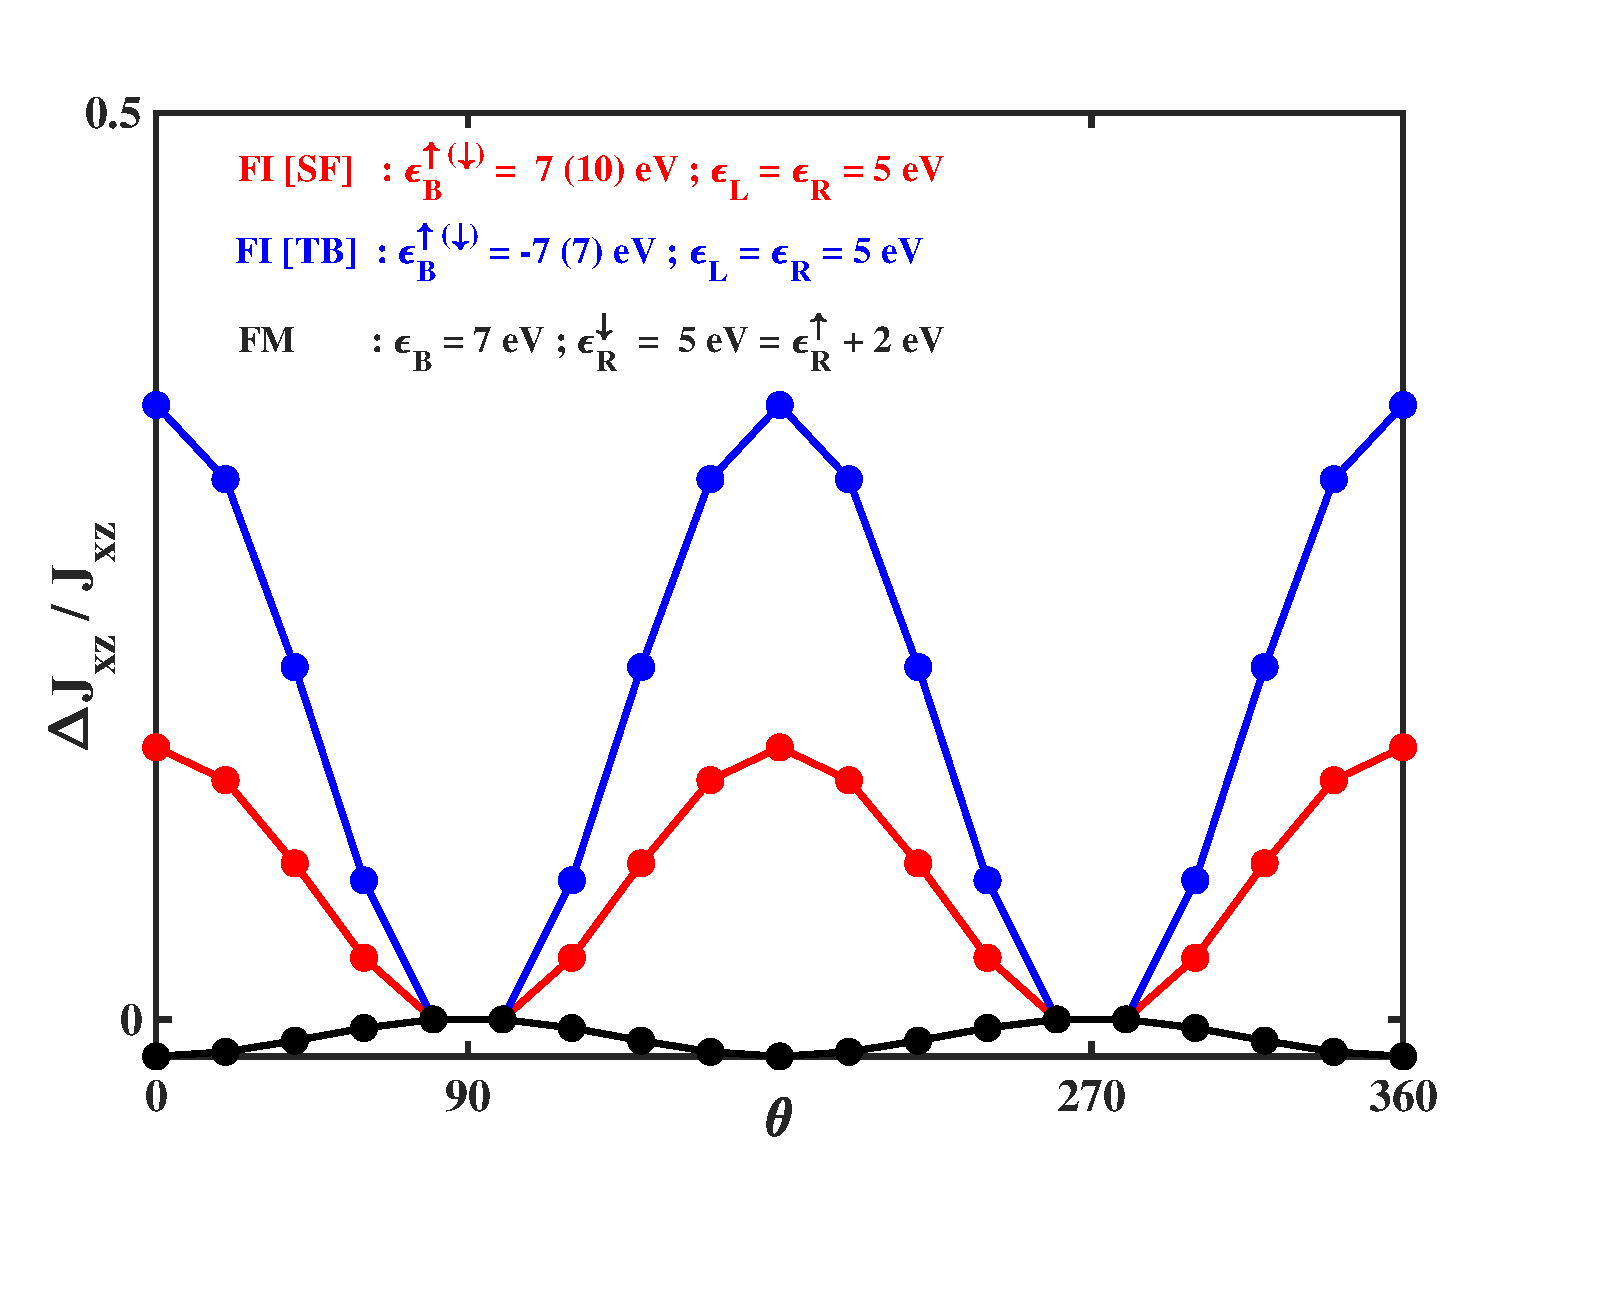
\includegraphics[width=0.8\columnwidth,clip=false]{fig4.eps}
\caption{(Online Color) The angular dependence of $\Delta J_{xz} /J_{xz}(\pi/2)$, with $\Delta J_{xz} = J_{xz}(0) -J_{xz}(\pi/2)$. In all cases, the contribution at zero bias is subtracted and therefore we use the upperindex \textit{net}. $\eps_L = \eps_{\rm R}^\upa$, $V = 0.5$ eV, $t = 1.0$ eV, and $\lambda = 0.05$ eV. Other parameters are given in the legend of the figure.}
\label{fig:figu4}
\end{figure}


\section{Conclusions}\label{sec:sec3}
In this study, we have examined the anomalous and spin Hall effects, tunneling anisotropic magnetoresistance (TAMR), and Rashba-induced spin-orbit torque in two distinct tunnel junction configurations: one involving a ferromagnetic insulator (NM/FI/NM) and the other featuring a ferromagnetic metal (NM/I/FM). For comparable barrier heights, ferromagnetic insulators present notable advantages over ferromagnetic metals. 
Firstly, TAMR becomes one order of magnitude larger when a ferromagnetic insulator is utilized instead of a ferromagnetic metal. This enhancement opens up possibilities for fabricating more efficient anisotropic sensors and memory devices. Notably, even with a decrease in the exchange splitting in the ferromagnetic barrier, the amplitude of TAMR remains larger than in semi-magnetic tunnel junctions, implying that ferromagnetic insulators with low exchange values, such as Eu chalcogenides and spinel-based materials, may suffice for achieving measurable TAMR values in practical applications.
From an experimental standpoint, this suggests that ferromagnetic insulators with low exchange values, such as Eu chalcogenides and spinel-based materials, may be sufficient to achieve measurable TAMR values for reliable applications. Furthermore, our findings pave the way for exploring novel approaches to increase TAMR, such as considering the surface states of heavy metals in contact with ferromagnetic insulators. These surface states can hybridize with bulk states, giving rise to surface resonances that can significantly enhance TAMR. 
Secondly, when examining the spin Hall effect, a similar outcome is observed in terms of its angular dependence. Although the spin Hall effect is larger in the presence of a ferromagnetic lead, its angular dependence becomes one order of magnitude larger when considering a ferromagnetic insulator. 
Lastly, the Rashba torque and the anomalous Hall effect exhibit similar characteristics in both types of systems, offering the possibility of fabricating single-magnetic-layer structures that are easier to implement without compromising the contribution of spin-orbit effects. These findings open up new avenues for exploring novel ferromagnetic insulators with larger exchange splittings and higher transition temperatures, potentially leading to more efficient devices compared to conventional semi-magnetic tunnel junctions.


\section*{ACKNOWLEDGMENTS}
C. O. P. acknowledge S. Nikolaev for insightful discussions.

\begin{thebibliography}{999}
\bibitem{rashba} A. Manchon, H. C. Koo, J. Nitta, S. M. Frolov, and R. A. Duine. 
\textit{New perspectives for Rashba spin-orbit coupling,}
\href{https://doi.org/10.1038/nmat4360}{Nat. Mat. {\bf 14}, 871 (2015).}

\bibitem{Soumyanarayanan2016} A. Soumyanarayanan, N. Reyren, A. Fert, and C. Panagopoulos, 
Emergent phenomena induced by spin-orbit coupling at surfaces and interfaces,
\href{https://www.nature.com/articles/nature19820}{Nature {\bf 539}, 509-517 (2016).} 

\bibitem{Manchon2019} A. Manchon, J. \u{Z}elezn\'y, I. M. Miron, T. Jungwirth, J. Sinova, A. Thiaville, K. Garello, and P. Gambardella, 
Current-induced spin-orbit torques in ferromagnetic and antiferromagnetic systems,
\href{https://journals.aps.org/rmp/abstract/10.1103/RevModPhys.91.035004}{Rev. Mod. Phys. {\bf 91}, 035004 (2019).}




\bibitem{sc} E. de Andrada e Silva, G. C. La Rocca, and F. Bassani. 
\textit{Spin split subbands and magneto-oscillations in III-V asymmetric heterostructures,}
\href{https://doi.org/10.1103/PhysRevB.50.8523}{Phys.Rev. B {\bf 50}, 8523 (1994).}
\textit{Spin-orbit splitting of electronic states in semiconductor asymmetric quantum wells,}
\href{https://doi.org/10.1103/PhysRevB.55.16293}{Phys. Rev. B {\bf 55}, 16293 (1997).}

\bibitem{miron} I. M. Miron, G. Gaudin, S. Auffret, B. Rodmacq, A. Schuhl, S. Pizzini, J. Vogel, and P. Gambardella. 
\textit{Current-driven spin torque induced by the Rashba effect in a ferromagnetic metal layer,}
\href{https://doi.org/10.1038/nmat2613}{Nat. Mat. {\bf 9}, 230 (2010). }

\bibitem{slg} A. Varykhalov, J. S\'anchez-Barriga, A. M. Shikin, C. Biswas, E. Vescovo, A. Rybkin, D. Marchenko, and O. Rader. 
\textit{Electronic and magnetic properties of quasifreestanding graphene on Ni,}
\href{https://doi.org/10.1103/PhysRevLett.101.157601}{Phys. Rev. Lett. {\bf 101}, 157601 (2008).}
Yu. S. Dedkov, M. Fonin, U. R\"udiger, and C. Laubschat.
\textit{Rashba effect in the graphene/Ni(111) system,}
\href{https://doi.org/10.1103/PhysRevLett.100.107602}{ Phys. Rev. Lett. {\bf 100}, 107602 (2008).}
Z. Y. Li, Z. Q. Yang, S. Qiao, J. Hu, and R. Q. Wu. 
\textit{Spin-orbit splitting in graphene on metallic substrates,}
\href{https://doi.org/10.1088/0953-8984/23/22/225502}{J. Phys.: Condens. Matter {\bf 23}, 225502 (2011).}
D. Marchenko, A. Varykhalov, M.R. Scholz, G. Bihlmayer, E.I. Rashba, A. Rybkin, A.M. Shikin, and O. Rader. 
\textit{Giant Rashba splitting in graphene due to hybridization with gold,}
\href{https://doi.org/10.1038/ncomms2227}{Nat. Commun. {\bf 3} 1232 (2012).}

\bibitem{ti} P. D. C. King, R. C. Hatch, M. Bianchi, R. Ovsyannikov, C. Lupulescu, G. Landolt, B. Slomski, J. H. Dil, D. Guan, J. L. Mi, E. D. L. Rienks, J. Fink, A. Lindblad, S. Svensson, S. Bao, G. Balakrishnan, B. B. Iversen, J. Osterwalder, W. Eberhardt, F. Baumberger, and Ph. Hofmann. 
\textit{Large tunable Rashba spin splitting of a two-dimensional electron gas in $\text{Bi}_2\text{Se}_3$,}
\href{https://doi.org/10.1103/PhysRevLett.107.096802}{Phys. Rev. Lett {\bf 107}, 096802 (2011).}

\bibitem{tmd} T. S. Ghiasi, A. A. Kaverzin, P. J. Blah, and B. J. van Wees. 
\textit{Charge-to-spin conversion by the Rashba-Edelstein effect in two-dimensional van der Waals heterostructures up to room temperature,}
\href{https://doi.org/10.1021/acs.nanolett.9b01611}{Nano Lett. {\bf 19} 5959 (2019).}

\bibitem{ahe-she} A. V. Vedyayev, M. S. Titova, N. V. Ryshanova, M. Y. Zhuravlev, and E. Y. Tsymbal. 
\textit{Anomalous and spin Hall effect in magnetic tunnel junction with Rashba spin-orbit coupling,}
\href{https://doi.org/10.1063/1.4815866}{Appl. Phys. Lett. {\bf 103}, 032406 (2013).}
A. Matos-Abiague and J. Fabian. 
\textit{Tunneling anomalous and spin Hall effects,}
\href{https://doi.org/10.1103/PhysRevLett.115.056602}{Phys. Rev. Lett. {\bf 115}, 056602 (2015).}

\bibitem{atmr0} A. Vedyayev, N. Ryzhanoca, N. Strelkov, M. Titova, M. Chshiev, B. Rodmacq, S. Auffret, L. Cuchet, L. Nistor, and B. Dieny. 
\textit{Influence of spin-orbit interaction within the insulating barrier on the electron transport in magnetic tunnel junctions,}
\href{https://doi.org/10.1103/PhysRevB.95.064420}{Phys. Rev. B {\bf 95}, 064420 (2017).}
 A. Matos-Abiague and J. Fabian. 
\textit{Anisotropic tunneling magnetoresistance and tunneling anisotropic magnetoresistance: Spin-orbit coupling in magnetic tunnel junctions,}
\href{https://doi.org/10.1103/PhysRevB.79.155303}{Phys. Rev. B {\bf 79}, 155303 (2009). }


\bibitem{tamr0} A. Matos-Abiague, M. Gmitra, and J. Fabian. 
\textit{Angular dependence of the tunneling anisotropic magnetoresistance in magnetic tunnel junctions,}
\href{https://doi.org/10.1103/PhysRevB.80.045312}{Phys. Rev. B {\bf 80}, 045312 (2009).}
J. Moser, A. Matos-Abiague, D. Schuh, W. Wegscheider, J. Fabian, and D. Weiss.
\textit{Tunneling anisotropic magnetoresistance and spin-orbit coupling in Fe/GaAs/Au tunnel junctions,}
\href{https://doi.org/10.1103/PhysRevLett.99.056601}{ Phys. Rev. Lett. {\bf 99}, 056601 (2007).}

\bibitem{half} J. D. Burton and E. Y. Tsymbal.
\textit{Tunneling anisotropic magnetoresistance in a magnetic tunnel junction with half-metallic electrodes,}
\href{https://doi.org/10.1103/PhysRevB.93.024419}{Phy. Rev. B {\bf 93}, 024419 (2016).}
Z. Quan, F. Zhang, Z. Yan, H. Liu, W. Zhang, B. Fang, G. Zhou, Z. Zeng, X. Xu.
\textit{Experimental observation of large tunneling anisotropic magnetoresistance in a magnetic tunnel junction without heavy metals,}
\href{https://doi.org/10.1016/j.apsusc.2020.146716}{J. Appl. Surf. Sci. 526, 146716 (2020).}



\bibitem{sot}
A. Manchon. 
\textit{Interfacial spin-orbit splitting and current-driven spin torque in anisotropic tunnel junctions,}
\href{https://doi.org/10.1103/PhysRevB.83.172403}{Phys. Rev. B {\bf 83}, 172403 (2011). }
K.-W. Kim, K.-J. Lee, J. Sinova, H.-W. Lee, and M. D. Stiles. 
\textit{Spin-orbit torques from interfacial spin-orbit coupling for various interfaces,}
\href{https://doi.org/10.1103/PhysRevB.96.104438}{Phys. Rev. B {\bf 96}, 104438 (2017).}

\bibitem{sp}
F. Mahfouzi, J. Fabian, N. Nagaosa, and B. K. Nikolic. 
\textit{Charge pumping by magnetization dynamics in magnetic and semimagnetic tunnel junctions with interfacial Rashba or bulk extrinsic spin-orbit coupling,}
\href{https://doi.org/10.1103/PhysRevB.85.054406}{Phys. Rev. B {\bf 85}, 054406 (2012).}







\bibitem{sf} J. S. Moodera. 
\textit{The phenomena of spin-filter tunneling,}
\href{https://doi.org/10.1088/0953-8984/19/16/165202}{J. Phys.: Condens. Matter {\bf 19}, 165202 (2007).}

\bibitem{magnon} L. J. Cornelissen, J. Liu, R. A. Duine, J. B. Youssef, and B. J. van Wees. 
\textit{Long-distance transport of mangon spin information in a magnetic insulator at room temperature,}
\href{https://doi.org/10.1038/nphys3465}{Nature Phys. {\bf 11}, 1022 (2015).}

\bibitem{Eu} G.-X. Miao, M. Muller, and J. S. Moodera. 
\textit{Magnetoresistance in double spin filter tunnel junctions with nonmagnetic electrodes and its unconventional bias dependence,}
\href{https://doi.org/10.1103/PhysRevLett.102.076601}{Phys. Rev. Lett. {\bf 102}, 076601 (2009). }
J. S. Moodera, R. Mersevey, and X. Hao. 
\textit{Variation of the electron-spin polarization in EuSe tunnel junctions from zero to near 100\% in a magnetic field,}
\href{https://doi.org/10.1103/PhysRevLett.70.853}{ Phys. Rev. Lett. {\bf 70}, 853 (1993).}
T. S. Santos and J. S. Moodera. 
\textit{Observation of spin filtering with a ferromagnetic EuO tunnel barrier,}
\href{https://doi.org/10.1103/PhysRevB.69.241203}{Phys. Rev. B {\bf 69} 241203(R) (2004).}

\bibitem{spinel} M. G. Chapline and S. X. Wang. 
\textit{Room-temperature spin filtering in a $Co$$Fe_2$$O_4$/Mg${Al}_{2}$$O_4$/$Fe_3$$O_4$ magnetic tunnel barrier,}
\href{https://doi.org/10.1103/PhysRevB.74.014418}{Phys. Rev. B {\bf 74}, 014418 (2006).}
U. Luders, M. Bibes, S. Fusil, K. Bouzehouane, E. Jacquet, C. B. Sommers, J.-P. Contour, J.-F. Bobo, A. Barth\'el\'emy, A. Fert, and P. M. Levy.
\textit{Bias dependence of tunnel magnetoresistance in spin filtering tunnel junctions: Experiment and theory,}
\href{https://doi.org/10.1103/PhysRevB.76.134412}{Phys. Rev B {\bf 76}, 134412 (2007). }
B. B. Nelson-Cheeseman, R. V. Chopdekar, L. M. B. Alldredge, J. S. Bettinger, E. Arenholz, and Y. Suzuki. 
\textit{Probing the role of the barrier layer in magnetic tunnel junction transport,}
\href{https://doi.org/10.1103/PhysRevB.76.220410}{Phys. Rev. B {\bf 76}, 220410(R) (2007). }
M. Gajek, M. Bibes, A. Barth\'el\'emy, K. Bouzehouane, S. Fusil, M. Varela, J. Fontcuberta, and A. Fert.  
\textit{Spin filtering through ferromagnetic BiMn$O_3$ tunnel barriers,}
\href{https://doi.org/10.1103/PhysRevB.72.020406}{Phys. Rev. B {\bf 72}, 020406(R) (2005).}
R. V. Chopdekar, B. B. Nelson-Cheeseman, M. Liberati, E. Arenholz, and Y. Suzuki. 
\textit{Role of magnetic anisotropy in spin-filter junctions,}
\href{https://doi.org/10.1103/PhysRevB.83.224426}{Phys. Rev B {\bf 83}, 224426 (2011).}

\bibitem{EuMR} G. Rimal and J. Tang.
\textit{Interface enhanced magnetic anisotropy in  $\text{Pt}/\text{EuO}_{1-x}$ films,}
\href{https://doi.org/10.1103/PhysRevB.98.144442}{Phys. Rev B {\bf 98}, 144442 (2018).}
K. Mallick, A. A. Wagh, A. Ionescu, C. H. W. Barnes, and P. S. A. Kumar.
\textit{Magnetoresistance effects in $\text{Pt}/\text{EuO}_{1-x}$,}
\href{https://doi.org/10.1063/5.0004049}{Appl. Phys. Lett. {\bf 116}, 202405 (2020).}

\bibitem{CoPt} B. G. Park, J. Wunderlich, D. A. Williams, S. J. Joo, K. Y. Jung, k. H. Shin, K. Olejnik, A. B. Shick, and T. Jungwirth.
\textit{Tunneling anisotropic magnetoresistance in multilayer-(Co/Pt)/$\text{AlO}_{x}$/P,}
\href{https://doi.org/10.1103/PhysRevLett.100.087204}{Phys. Rev. Lett. {\bf 100}, 087204 (2008).}


\bibitem{Zalto2023}
V. Zatko, R. Galceran, M. Galbiati, J. Peiro, F. Godel, L.-M. Kern, D. Perconte, F. Ibrahim, A. Hallal, M. Chshiev, B. Martinez, C. Frontera, L. Balcells, P. R. Kidambi, J. Robertson, S. Hofmann, S. Collin, F. Petroff, M.-B. Martin, B. Dlubak, and P. Seneor, 
Artificial Graphene Spin Polarized Electrode for Magnetic Tunnel Junctions
\href{https://pubs.acs.org/doi/full/10.1021/acs.nanolett.2c03113}{Nano Lett. 23, 1, 34-41 (2023).}




\bibitem{tamr1} L. Lopez-Mir, C. Frontera, H. Aramberri, K. Bouzehouane, J. Cisneros-Fernandez, B. Bozzo, L. Balcells, and B. Martinez. 
\textit{Anisotropic sensor and memory device with a ferromagnetic tunnel barrier as the only magnetic element}
\href{https://doi.org/10.1038/s41598-017-19129-5}{Sci. Rep. {\bf 8}, 861 (2018).}

\bibitem{ahe1} M. Ye. Zhuravlev, A. V. Vedyayev, M. S. Titova, N. V. Ryzhanova, and D. Gusakova.
\textit{Surface current at non-magnetic metal/ferromagnetic insulator interfacedue to Rashba spin-orbit interaction}
\href{https://doi.org/10.1016/j.jmmm.2017.06.044}{J. of Magn. and Mag. Mat. {\bf 441} 572 (2017).}


\bibitem{Solis2019} D. A. Solis, A. Hallal, X. Waintal, and M. Chshiev, 
Proximity magnetoresistance in graphene induced by magnetic insulators
\href{https://journals.aps.org/prb/abstract/10.1103/PhysRevB.100.104402}{Phys. Rev. B {\bf 100}, 104402 (2019).}


\bibitem{Hallal2017} A. Hallal, F. Ibrahim, H. Yang, S. Roche, and M. Chshiev,
Tailoring magnetic insulator proximity effects in graphene: first-principles calculations
\href{https://iopscience.iop.org/article/10.1088/2053-1583/aa6663}{2D Mater. {\bf 4}, (2017).}



\bibitem{kohn}
W. Kohn, L. J. Sham, \emph{Self-Consistent Equations Including Exchange and Correlation Effects}, 
\href{https://journals.aps.org/pr/abstract/10.1103/PhysRev.140.A1133}{Phys. Rev. A \textbf{140}, 1133 (1965).}

\bibitem{gga}
J. P. Perdew, K. Burke, and M. Ernzerhof, \emph{Generalized Gradient Approximation Made Simple}, 
\href{https://journals.aps.org/prl/abstract/10.1103/PhysRevLett.77.3865}{Phys. Rev. Lett. \textbf{77}, 3865 (1996).}















\bibitem{paw}
P. E. Blochl, \emph{Projector augmented-wave method}, 
\href{https://journals.aps.org/prb/abstract/10.1103/PhysRevB.50.17953}{Phys. Rev. B \textbf{50}, 17953 (1994).}

\bibitem{vasp}
G. Kresse, J. Hafner, \emph{Ab-initio molecular dynamics for liquid metals}, 
\href{https://journals.aps.org/prb/abstract/10.1103/PhysRevB.47.558}{Phys. Rev. B \textbf{47}, 558 (1993).}


\bibitem{Kresse1994} G. Kresse and J. Hafner, 
Ab initio molecular-dynamics simulation of the liquid-metal–amorphous-semiconductor transition in germanium
\href{https://journals.aps.org/prb/abstract/10.1103/PhysRevB.49.14251}{Phys. Rev. B {\bf 49} , 14251 (1994).}


\bibitem{Kresse1996a}
G. Kresse and J. Furthmuller, 
Efficiency of ab-initio total energy calculations for metals and semiconductors using a plane-wave basis set, 
\href{https://www.sciencedirect.com/science/article/abs/pii/0927025696000080}{Comput. Mat. Sci. {\bf 6} , 15 (1996).} 

\bibitem{Kresse1996b} 
G. Kresse and J. Furthmuller, 
Efficient iterative schemes for ab initio total-energy calculations using a plane-wave basis set,
\href{https://journals.aps.org/prb/abstract/10.1103/PhysRevB.54.11169}{Phys. Rev. B {\bf }54 , 11169 (1996).}




\bibitem{mppoint}
H. J. Monkhorst, J. D. Pack, \emph{Special points for Brillouin-zone integrations}, 
\href{https://journals.aps.org/prb/abstract/10.1103/PhysRevB.13.5188}{Phys. Rev. B \textbf{13}, 5188 (1976).}

\bibitem{ldau}
A. I. Liechtenstein, V. I. Anisimov and J. Zaanen, \emph{Density-functional theory and strong interactions: Orbital ordering in Mott-Hubbard insulators}, 
\href{https://journals.aps.org/prb/abstract/10.1103/PhysRevB.52.R5467}{Phys. Rev. B \textbf{52}, R5467 (1995).}



\bibitem{Yang2013} 
H. X. Yang, A. Hallal, D. Terrade, X. Waintal, S. Roche, and M. Chshiev,
Proximity Effects Induced in Graphene by Magnetic Insulators: First-Principles Calculations on Spin Filtering and Exchange-Splitting Gaps, 
\href{https://journals.aps.org/prl/abstract/10.1103/PhysRevLett.110.046603}{Phys. Rev. Lett. {\bf 110}, 046603 (2013).}

\bibitem{Ingle2008}
 N. J. C. Ingle and I. S. Elfimov, 
Influence of epitaxial strain on the ferromagnetic semiconductor EuO: First-principles calculations, 
\href{https://journals.aps.org/prb/abstract/10.1103/PhysRevB.77.121202}{Phys. Rev. B {\bf 77}, 121202(R) (2008).}


\bibitem{Shubin1934} S. P. Shubin and S. V. Vonsovski,
On the electron theory of metals, 
\href{https://royalsocietypublishing.org/doi/10.1098/rspa.1934.0089}{Proc. Roy. Soc. A145, 159 (1934)}; 
S.V. Vonsovski, Magnetism (Wiley, New York, 1974).



\bibitem{fifm}
For a system of the form FI/FM we fix the magnetic layer in the barrier along the $z-$ axis, i.e., $\theta_{\rm B} = 0$. Then we have,
\begin{align}
\label{jxxoo}
j_{x}^{\rm soc} &=  \lam\xi \frac{ \dlt_q \Sg_k\Sg_q +\dlt_k(2k_{\rm R}^\dna k_{\rm R}^\upa-q_{\rm R}^{2\downarrow}-q_{\rm R}^{2\uparrow})\cos\theta_{\rm R}}{D_\theta/4}, \\
\label{jzzoo}
j_{z}^{\rm soc} &=\lam\xi \frac{\dlt_k(q_{\rm R}^\downarrow q_{\rm R}^\uparrow -k_{\rm R}^{\dna} k_{\rm R}^\upa )\sin \theta_{\rm R} \cos\phi_{\rm R}}{D_\theta/8} , \\
J_{xz}^{\rm soc} &=   \lam\frac{\Sg_k (q_{\rm R}^{2\downarrow}+q_{\rm R}^{2\uparrow}+2k_{\rm R}^\dna k_{\rm R}^\upa)-\dlt_k\dlt_q \Sg_q\cos\theta_{\rm R}}{D_\theta/2},  
\label{jxzoo}
\end{align}


with $D_\theta=4(q_{\rm R}^\uparrow q_{\rm R}^\downarrow-k_{\rm R}^\uparrow k_{\rm R}^\downarrow)^2+(\Sg_k \Sg_q -\dlt_k\dlt_q\cos\theta_{\rm R})^2$. As seen in Eq. \eqref{jxzoo}, the spin current density acquires an angular dependence to the first order in Rashba SOC.

\bibitem{vedyayev_prl} A. Vedyayev, N. Ryshanova, N. Strelkov, and B. Dieny. 
\textit{Spontaneous anomalous and spin Hall effects due to spin-orbit scattering of evanescent wave functions in magnetic tunnel junctions}
\href{https://doi.org/10.1103/PhysRevLett.110.247204}{Phys. Rev. Lett. {\bf 110}, 247204 (2013).}
\bibitem{atmr}
Only one spin-band is considered in a ferromagnetic barrier, then,
\begin{align}
\beta_0 &= \big{[}k_{\rm R}^{\dna 2} k_{\rm R}^{\upa 2} ( 3 q_{\rm R}^2 - k_{\rm R}^{\dna } k_{\rm R}^{\upa }) +q_{\rm R}^4(  7 k_{\rm R}^\dna k_{\rm R}^\upa - 5 q_{\rm R}^2 )  +\nn\\
&  ~~~~~ q_{\rm R}^2(k_{\rm R}^{\dna 2} + k_{\rm R}^{\upa 2})(3 k_{\rm R}^\dna k_{\rm R}^\upa - q_{\rm R}^2)\big{]} / (k_{\rm R}^\upa k_{\rm R}^\dna + q_{\rm R}^2), \\
\beta_0^* &= \big{[}q_{\rm R}^{\upa 2} (3 q_{\rm R}^{\dna} + q_{\rm R}^\upa) - k_{\rm R}^2 (3 q_{\rm R}^\upa +q_{\rm R}^{\dna})\big{]} (k_{\rm R}^2 + q_{\rm R}^{\dna 2})  
\end{align}

\bibitem{kalitsov} A. Kalitsov, M. Chshiev, I. Theodonis, N. Kioussis, and W. H. Butler
\textit{Spin-transfer torque in magnetic tunnel junctions}
\href{https://doi.org/10.1103/PhysRevB.79.174416}{Phys. Rev. B {\bf 79}, 174416 (2009).}

\bibitem{CoFeB} S. Hatanaka, S. Miwa, K. Matsuda, K. Nawaoka, K. Tanaka, H. Morishita, M. Goto, N. Mizuochi, T. Shinjo, and Y. Suzuki
\textit{Tunneling anisotropoc magnetoresistance in CoFeB/MgO/Ta junctions}
\href{https://doi.org/10.1063/1.4929682}{Appl. Phys. Lett. {\bf 107}, 082407 (2015).}

\bibitem{cop} C. Ortiz Pauyac, A. Kalitsov, A. Manchon, and M. Chshiev
\textit{Spin-transfer torque in spin filter tunnel junctions}
\href{https://doi.org/10.1103/PhysRevB.90.235417}{Phys. Rev. B {\bf 90}, 235417 (2014).}

\bibitem{surface} A. N. Chantis, K. D. Belashchenko, E. Y. Tsymbal, and M. van Schilfgaarde.
\textit{Tunneling anisotropic magnetoresistance driven by resonant surface states: First-principles calculations on a Fe(001) surface,}
\href{https://doi.org/10.1103/PhysRevLett.98.046601}{Phys. Rev. Lett. {\bf 98}, 046601 (2007).}
\end{thebibliography}
\end{document}
